% !TeX program = xelatex
% !TeX encoding = UTF-8
% Spedizione P01 · Geometria dei pori e permeabilità
% Presentazione della spedizione P01 nella serie planetaria di GeoStat Lab.
% Compilazione: xelatex -interaction=nonstopmode P01_Pori.tex (due passaggi)
% 31 slide. Diagrammi TikZ, figure vettoriali da R/P01_figure.R, codice R, dati ed esperimenti inclusi.
\RequirePackage{fix-cm}
\documentclass[12pt,aspectratio=1610]{beamer}
\geometry{paperwidth=20cm,paperheight=12.5cm}
\usepackage[italian,provide=*]{babel}
\usepackage{fontspec,adjustbox,tabularx}
\IfFontExistsTF{NimbusSans-Regular.otf}{
\setsansfont{NimbusSans-Regular.otf}[BoldFont=NimbusSans-Bold.otf,ItalicFont=NimbusSans-Italic.otf,BoldItalicFont=NimbusSans-BoldItalic.otf]
\setmainfont{NimbusSans-Regular.otf}[BoldFont=NimbusSans-Bold.otf,ItalicFont=NimbusSans-Italic.otf,BoldItalicFont=NimbusSans-BoldItalic.otf]
}{
\setsansfont{TeX Gyre Heros}
\setmainfont{TeX Gyre Heros}
}
\IfFontExistsTF{DejaVu Sans Mono}{
\setmonofont{DejaVu Sans Mono}[Scale=.88]
}{\setmonofont{Latin Modern Mono}[Scale=.88]}
\usefonttheme{professionalfonts}
\usepackage{amsmath,amssymb,booktabs,array,graphicx,tikz,bookmark}
\usetikzlibrary{calc,positioning,arrows.meta}
\graphicspath{{Figure/}}
\definecolor{Paper}{HTML}{F8F6F1}
\definecolor{Ink}{HTML}{253344}
\definecolor{Navy}{HTML}{15283E}
\definecolor{Quantum}{HTML}{5146A5}
\definecolor{Classical}{HTML}{087C74}
\definecolor{Muted}{HTML}{657180}
\definecolor{Rule}{HTML}{D6DAD9}
\definecolor{Night}{HTML}{112236}
\definecolor{Lilac}{HTML}{ABB5FF}
\definecolor{Mint}{HTML}{72D8C8}
\setbeamercolor{background canvas}{bg=Paper}
\setbeamercolor{normal text}{fg=Ink}
\setbeamertemplate{navigation symbols}{}
\setbeamertemplate{headline}{}
\setbeamertemplate{footline}{}
\setbeamersize{text margin left=0pt,text margin right=0pt}
\hypersetup{colorlinks=true,linkcolor=Classical,urlcolor=Classical,pdfpagemode=UseOutlines,pdfstartview=Fit,
 pdftitle={Spedizione P01 · Geometria dei pori e permeabilità},pdfauthor={GeoStat Lab · materiali di Marzio De Corato},
 pdfsubject={GeoStat Lab · P01}}
\bookmarksetup{open,openlevel=0,depth=2}
\newsavebox{\BodyBox}
\newsavebox{\SideBox}
\newsavebox{\RecallBox}
\newsavebox{\TitleBox}
\newcommand{\MeasureBox}[2]{\typeout{REVIEWBOX:#1:\the\wd#2:\the\ht#2:\the\dp#2}}

% Revisione completa: diagrammi TikZ, formalismo e box R.
\usepackage[most]{tcolorbox}
\usepackage{listings}
\usetikzlibrary{fit,backgrounds,matrix,decorations.pathreplacing}
\definecolor{GeoA}{HTML}{1D7890}
\definecolor{GeoB}{HTML}{C57E42}
\definecolor{GeoC}{HTML}{7363AA}
\definecolor{GeoTint}{HTML}{F0F4F3}
\lstdefinestyle{GeoR}{language=R,basicstyle=\ttfamily\fontsize{9.2}{12.2}\selectfont,
 keywordstyle=\color{Quantum}\bfseries,commentstyle=\color{Classical},stringstyle=\color{GeoB},
 numbers=left,numberstyle=\tiny\color{Muted},numbersep=4pt,showstringspaces=false,
 columns=fullflexible,keepspaces=true,breaklines=true,xleftmargin=1.15em,
 frame=none,aboveskip=0pt,belowskip=0pt,tabsize=2}
\newsavebox{\PilotLeftBox}
\newsavebox{\PilotRightBox}
\newcommand{\PLabel}[1]{\par{\color{Classical}\bfseries\fontsize{9}{11}\selectfont\MakeUppercase{#1}}\par\vspace{1.8mm}}
\newcommand{\PBody}[1]{\par{\fontsize{11.3}{14.8}\selectfont #1\par}}
\newcommand{\PSmall}[1]{\par{\fontsize{9.8}{13.1}\selectfont #1\par}}
\newcommand{\PCode}[2]{%
\begin{tcolorbox}[enhanced,arc=1.8mm,boxrule=.65pt,
  colback=white,colframe=Classical!75!Navy,colbacktitle=Navy,
  coltitle=white,fonttitle=\bfseries\fontsize{9.6}{12}\selectfont,
  title={#1},left=1.7mm,right=1.3mm,top=1.5mm,bottom=1.3mm,
  before skip=1mm,after skip=1mm]
\lstinputlisting[style=GeoR]{Codice/#2}
\end{tcolorbox}}
\newcommand{\PInfo}[1]{%
\begin{tcolorbox}[enhanced,arc=1.6mm,boxrule=.55pt,colback=GeoTint,
 colframe=Rule!80!Classical,left=2.3mm,right=2.3mm,top=2mm,bottom=2mm,
 before skip=1mm,after skip=1mm]
\PSmall{#1}\end{tcolorbox}}
\tikzset{
 pFlow/.style={draw=Classical!45,fill=white,rounded corners=2mm,
  line width=.7pt,align=center,minimum height=1.1cm,font=\sffamily\fontsize{10}{12}\selectfont},
 pEdge/.style={-{Latex[length=2.3mm]},draw=Classical,line width=.95pt},
 pGroup/.style={draw=Rule,fill=white,rounded corners=2mm,line width=.65pt},
 pDotA/.style={circle,fill=GeoA,inner sep=1.25pt},
 pDotB/.style={circle,fill=GeoB,inner sep=1.25pt},
 pDotC/.style={circle,fill=GeoC,inner sep=1.25pt}
}
\newcommand{\PilotChrome}[4]{%
  \node[anchor=north west,inner sep=0,text width=17.7cm] at ([xshift=.95cm,yshift=-.55cm]current page.north west) {\color{Navy}\bfseries\fontsize{20.6}{24.5}\selectfont #1};
  \node[anchor=north east,inner sep=0] at ([xshift=19.05cm,yshift=-.14cm]current page.north west) {\color{Classical}\fontsize{8}{10}\selectfont\hyperlink{slide2}{#2}};
  \draw[Classical,line width=1.2pt] ([xshift=.95cm,yshift=-1.7cm]current page.north west)--([xshift=2.35cm,yshift=-1.7cm]current page.north west);
  \draw[Rule,line width=.65pt] ([xshift=.95cm,yshift=-10.36cm]current page.north west)--([xshift=19.05cm,yshift=-10.36cm]current page.north west);
  \node[anchor=north west,inner sep=0] at ([xshift=.96cm,yshift=-10.55cm]current page.north west) {\color{Classical}\bfseries\fontsize{9.1}{12}\selectfont DA RICORDARE};
  \node[anchor=north west,inner sep=0,text width=14.3cm] at ([xshift=4.2cm,yshift=-10.53cm]current page.north west) {\color{Ink}\fontsize{10.3}{13.8}\selectfont #4};
  \draw[Rule,line width=.35pt] ([xshift=.95cm,yshift=-11.92cm]current page.north west)--([xshift=19.05cm,yshift=-11.92cm]current page.north west);
  \node[anchor=north west,inner sep=0] at ([xshift=.95cm,yshift=-12.06cm]current page.north west) {\color{Muted}\fontsize{7.7}{9.2}\selectfont Spedizione P01 · Geometria dei pori e permeabilità};
  \node[anchor=north east,inner sep=0] at ([xshift=19.05cm,yshift=-12.06cm]current page.north west) {\color{Muted}\fontsize{7.7}{9.2}\selectfont #3/31};
}


% Stili comuni per i diagrammi scientifici della revisione completa.
\tikzset{
 pAxis/.style={-{Latex[length=2mm]},draw=Muted,line width=.65pt},
 pNote/.style={font=\sffamily\fontsize{9}{11.5}\selectfont,text=Muted,align=center},
 pLabel/.style={font=\sffamily\fontsize{10}{12.5}\selectfont,text=Ink,align=center}
}
\newsavebox{\FullWideBox}
\setlength{\emergencystretch}{1em}




\newcommand{\PLab}[2]{\par{\color{Classical}\bfseries\fontsize{9}{11}\selectfont
\href{#1}{\MakeUppercase{#2}}}\par\vspace{1.8mm}}

\definecolor{Measure}{HTML}{A05B10}\definecolor{Rose}{HTML}{9B4564}\definecolor{Wash}{HTML}{EAE7F6}\definecolor{Gold}{HTML}{EEC184}
\tikzset{arr/.style={-{Stealth[length=2mm]},line width=.8pt,draw=Classical}}
\newcommand{\Colonna}[2]{\begin{adjustbox}{max totalsize={#1}{7.95cm},valign=t}\begin{minipage}[t]{#1}\raggedright\fontsize{11.3}{14.8}\selectfont #2\end{minipage}\end{adjustbox}}
\begin{document}

\begin{frame}[plain]\hypertarget{slide1}{}\bookmark[level=0,page=1]{Spedizione P01}
\begin{tikzpicture}[remember picture,overlay]
\fill[Night](current page.south west) rectangle(current page.north east);
\IfFileExists{Scena/copertina.jpg}{\node[inner sep=0] at(current page.center){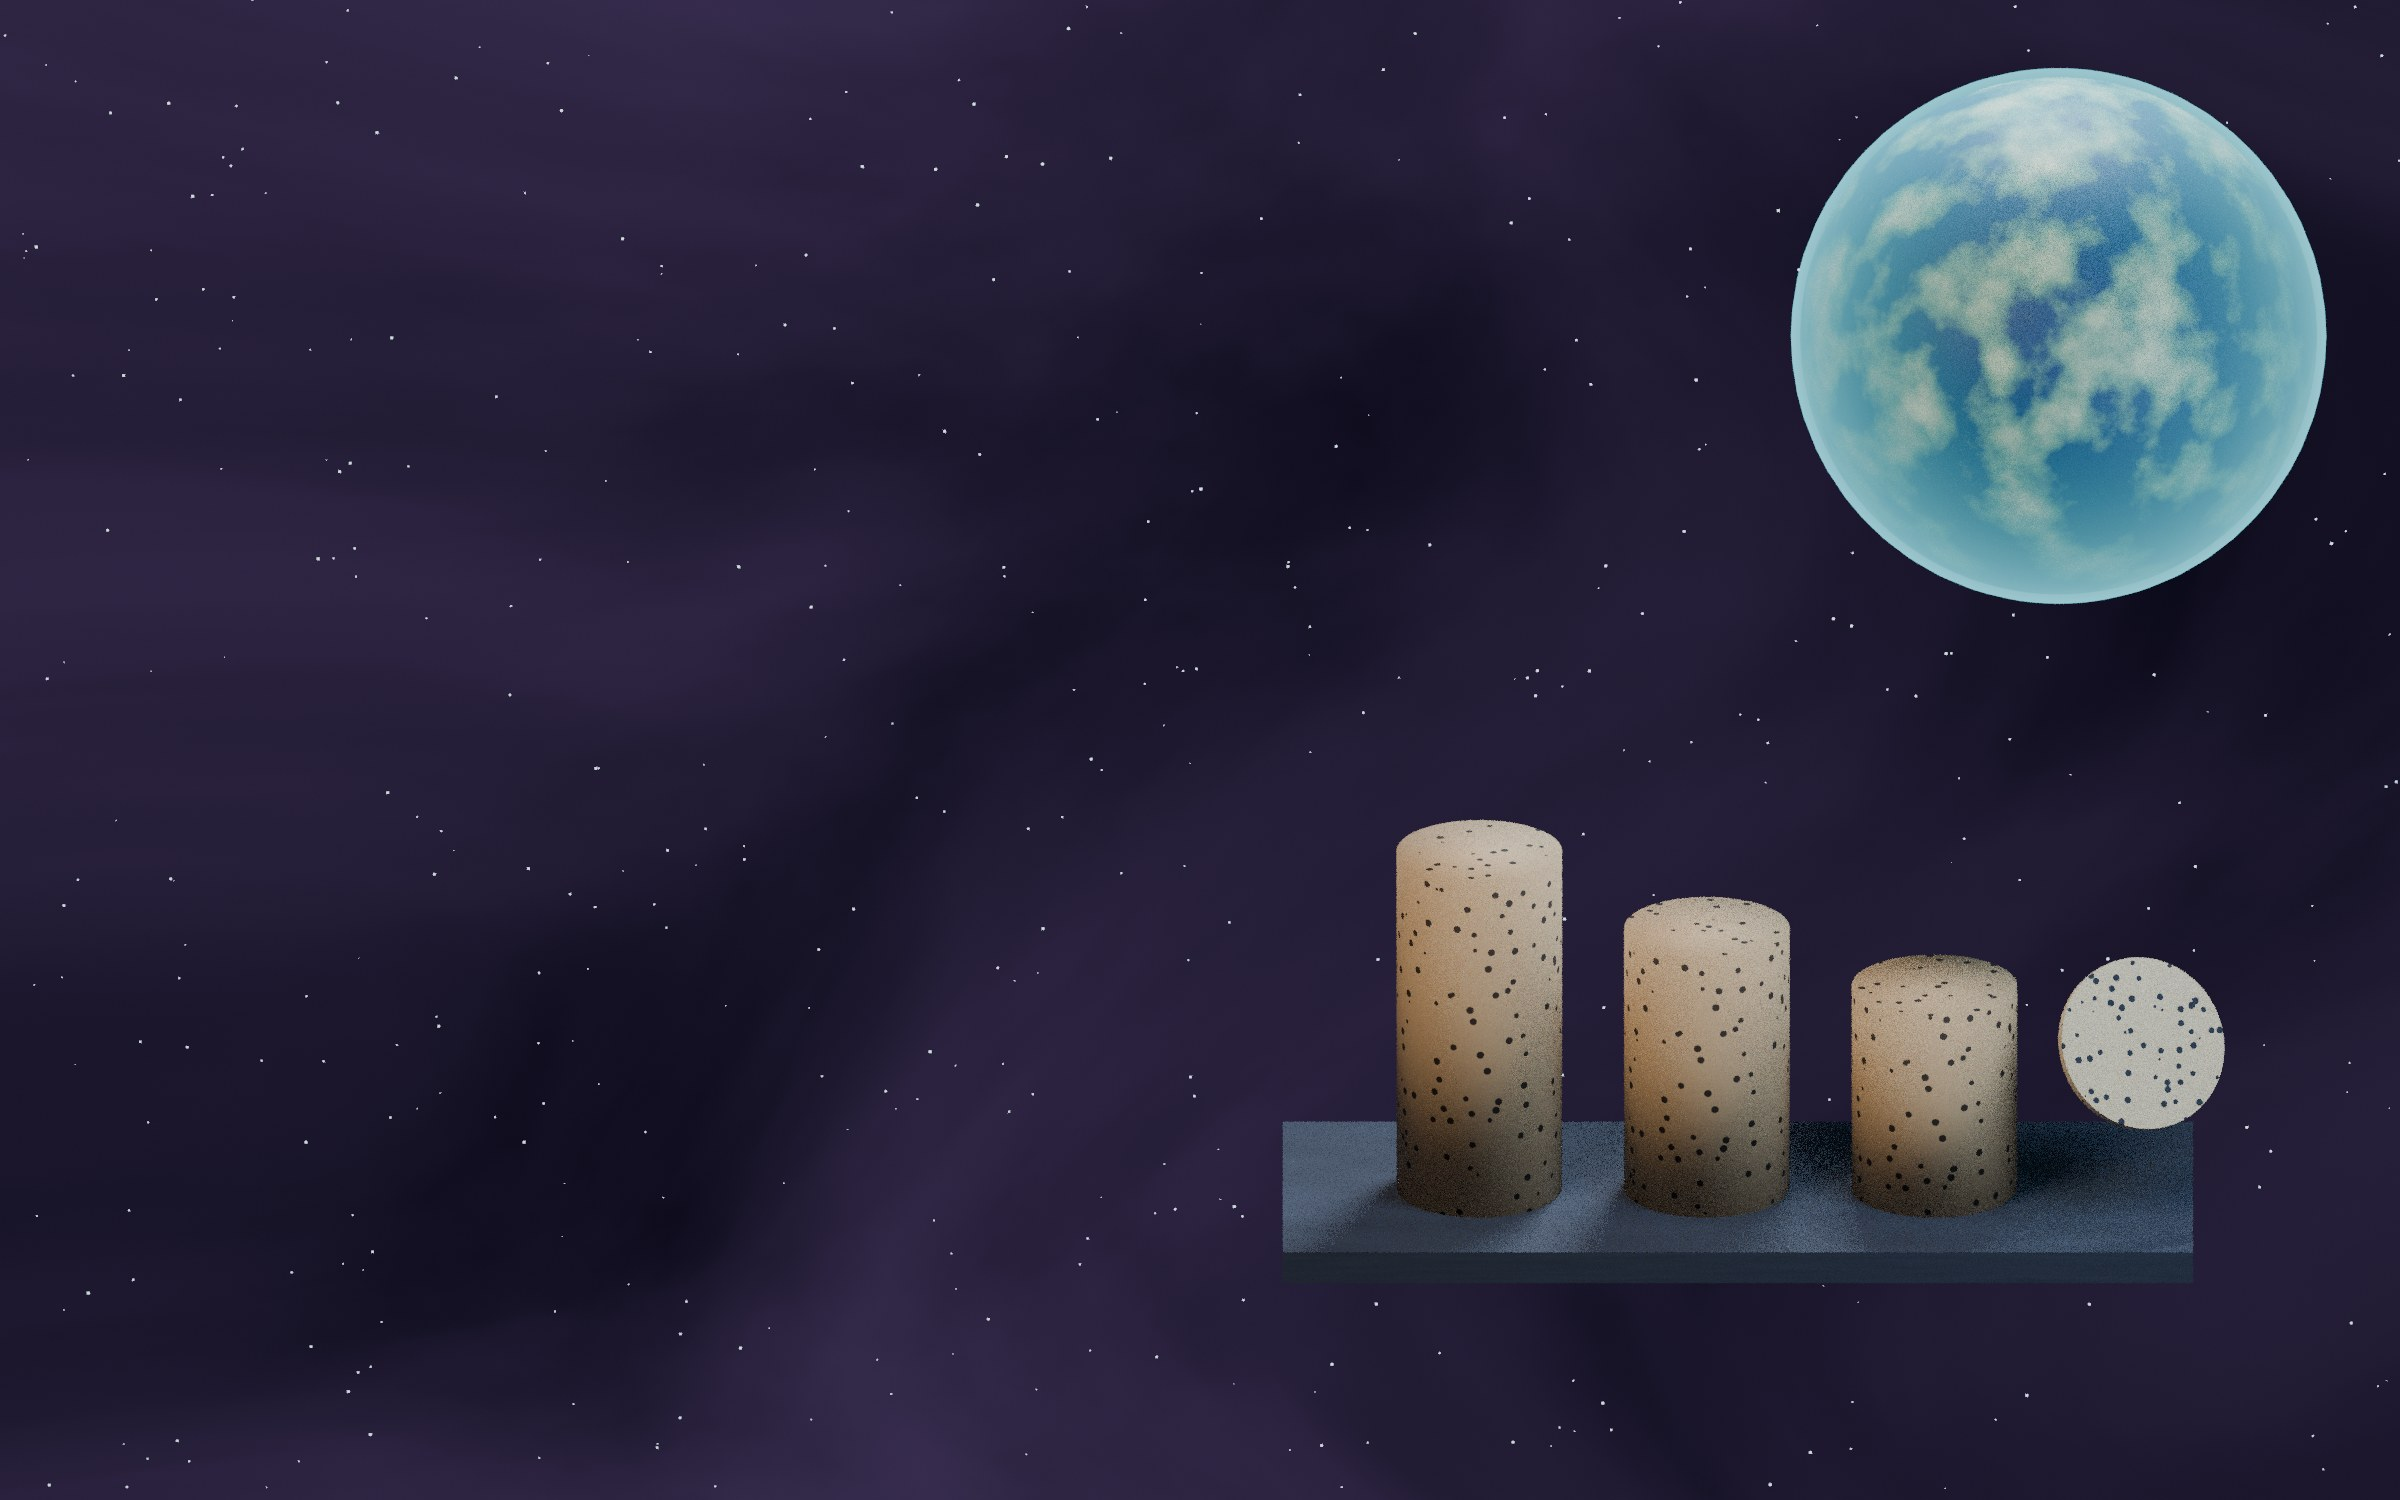
\includegraphics[width=20cm,height=12.5cm]{Scena/copertina.jpg}};}{}
\node[anchor=north west,inner sep=0] at([xshift=1.05cm,yshift=-1.10cm]current page.north west){\color{Mint}\bfseries\fontsize{23}{28}\selectfont SPEDIZIONE P01};
\node[anchor=north west,inner sep=0] at([xshift=1.07cm,yshift=-2.16cm]current page.north west){\color{white}\fontsize{9}{12}\selectfont MACROPROGETTO P01 · SCIENZE DELLA TERRA};
\draw[Mint,line width=1.5pt]([xshift=1.07cm,yshift=-2.78cm]current page.north west)--([xshift=2.6cm,yshift=-2.78cm]current page.north west);
\node[anchor=north west,inner sep=0] at([xshift=1.05cm,yshift=-3.35cm]current page.north west){\begin{minipage}{9.2cm}\raggedright\color{white}\bfseries\fontsize{28.5}{34.5}\selectfont Geometria dei pori\\e permeabilità\end{minipage}};
\node[anchor=north west,inner sep=0] at([xshift=1.07cm,yshift=-7.88cm]current page.north west){\begin{minipage}{8.9cm}\raggedright\color{Lilac}\fontsize{12.2}{17}\selectfont Dodici carote, quarantotto sezioni\end{minipage}};
\node[anchor=north west,inner sep=0] at([xshift=1.07cm,yshift=-8.70cm]current page.north west){\begin{minipage}{8.9cm}\raggedright\color{white!75}\fontsize{10.3}{14.5}\selectfont Sezioni, carote e inferenza su un piccolo campione osservativo\end{minipage}};
\node[anchor=north west,inner sep=0] at([xshift=1.07cm,yshift=-10.52cm]current page.north west){\color{white}\fontsize{10.5}{14}\selectfont GeoStat Lab · corso di Marzio De Corato};
\node[anchor=north west,inner sep=0] at([xshift=1.07cm,yshift=-11.17cm]current page.north west){\color{Mint}\fontsize{8.8}{11}\selectfont\href{https://creativecommons.org/licenses/by-nc-sa/4.0/}{Impaginazione da Tessera · CC BY-NC-SA 4.0}};
\end{tikzpicture}\end{frame}

\begin{frame}[plain]\hypertarget{slide2}{}
\bookmark[level=1,page=2]{Indice della presentazione}
\begin{tikzpicture}[remember picture,overlay]
\PilotChrome{Indice della presentazione}{PERCORSO}{2}{I titoli dell’indice aprono i capitoli. Il nome del capitolo in alto riporta a questa pagina.}
\node[anchor=north west,inner sep=0] at([xshift=.96cm,yshift=-2.12cm]current page.north west){\Colonna{9.40cm}{\PLabel{Capitoli}
{\fontsize{10.7}{13.5}\selectfont\hyperlink{slide4}{Domanda geologica e supporto della misura\hfill 4}\par}\vspace{.16cm}
{\fontsize{10.7}{13.5}\selectfont\hyperlink{slide9}{Visualizzazione e unità di analisi\hfill 9}\par}\vspace{.16cm}
{\fontsize{10.7}{13.5}\selectfont\hyperlink{slide11}{Modello e interpretazione del parametro\hfill 11}\par}\vspace{.16cm}
{\fontsize{10.7}{13.5}\selectfont\hyperlink{slide16}{Ricampionamento e sensibilità\hfill 16}\par}\vspace{.16cm}
{\fontsize{10.7}{13.5}\selectfont\hyperlink{slide21}{Argomentazione geologica e consegna\hfill 21}\par}\vspace{.16cm}
{\fontsize{10.7}{13.5}\selectfont\hyperlink{slide23}{Laboratori della spedizione\hfill 23}\par}\vspace{.16cm}

}};
\node[anchor=north west,inner sep=0] at([xshift=10.85cm,yshift=-2.12cm]current page.north west){\Colonna{8.16cm}{\PLabel{Percorso di lettura}
\PBody{Il percorso parte dal supporto delle misure, costruisce una sintesi per carota, stima la pendenza in scala logaritmica e ne esamina la stabilità. I laboratori finali riprendono le tre fasi della spedizione.}
\PInfo{Le pagine Scenario A e Confronto riprendono gli esperimenti nel browser con dati sintetici. I valori di partenza del simulatore differiscono da quelli del caso.}
\href{https://marzione00.github.io/Lab_Geo/\#modulo-P01}{\color{Classical}\bfseries Apri la spedizione P01 su GeoStat Lab}
}};
\end{tikzpicture}\end{frame}

\begin{frame}[plain]\hypertarget{slide3}{}
\bookmark[level=1,page=3]{Come varia la permeabilità di una carota con la frazione areale dei suoi pori?}
\begin{tikzpicture}[remember picture,overlay]
\PilotChrome{{\fontsize{15.3}{19}\selectfont Come varia la permeabilità di una carota con la frazione areale dei suoi pori?}}{IL CASO GUIDA}{3}{La copertina è una scena illustrativa. I valori analizzati provengono dal dataset rock distribuito con R.}
\node[anchor=north west,inner sep=0] at([xshift=.96cm,yshift=-2.12cm]current page.north west){\Colonna{9.40cm}{{\centering\resizebox{0.97\linewidth}{!}{\begin{tikzpicture}[x=1cm,y=1cm,every node/.style={font=\sffamily\fontsize{10}{12}\selectfont,text=Ink}]
\draw[draw=Classical,fill=Classical!8,rounded corners=2mm,line width=.7pt] (0,0.00) rectangle (8.6,-0.78);
\node[circle,anchor=center,fill=Classical,inner sep=0,minimum size=.5cm,text=white,font=\sffamily\bfseries\fontsize{9}{10}\selectfont] at (.48,-0.39) {1};
\node[anchor=west,text width=7.4cm,align=left] at (.95,-0.39) {Domanda geologica e supporto della misura};
\draw[pEdge] (.48,-0.80)--(.48,-1.02);
\draw[draw=Classical,fill=Classical!8,rounded corners=2mm,line width=.7pt] (0,-1.04) rectangle (8.6,-1.82);
\node[circle,anchor=center,fill=Classical,inner sep=0,minimum size=.5cm,text=white,font=\sffamily\bfseries\fontsize{9}{10}\selectfont] at (.48,-1.43) {2};
\node[anchor=west,text width=7.4cm,align=left] at (.95,-1.43) {Visualizzazione e unità di analisi};
\draw[pEdge] (.48,-1.84)--(.48,-2.06);
\draw[draw=Classical,fill=Classical!8,rounded corners=2mm,line width=.7pt] (0,-2.08) rectangle (8.6,-2.86);
\node[circle,anchor=center,fill=Classical,inner sep=0,minimum size=.5cm,text=white,font=\sffamily\bfseries\fontsize{9}{10}\selectfont] at (.48,-2.47) {3};
\node[anchor=west,text width=7.4cm,align=left] at (.95,-2.47) {Modello e interpretazione del parametro};
\draw[pEdge] (.48,-2.88)--(.48,-3.10);
\draw[draw=Classical,fill=Classical!8,rounded corners=2mm,line width=.7pt] (0,-3.12) rectangle (8.6,-3.90);
\node[circle,anchor=center,fill=Classical,inner sep=0,minimum size=.5cm,text=white,font=\sffamily\bfseries\fontsize{9}{10}\selectfont] at (.48,-3.51) {4};
\node[anchor=west,text width=7.4cm,align=left] at (.95,-3.51) {Ricampionamento e sensibilità};
\draw[pEdge] (.48,-3.92)--(.48,-4.14);
\draw[draw=Classical,fill=Classical!8,rounded corners=2mm,line width=.7pt] (0,-4.16) rectangle (8.6,-4.94);
\node[circle,anchor=center,fill=Classical,inner sep=0,minimum size=.5cm,text=white,font=\sffamily\bfseries\fontsize{9}{10}\selectfont] at (.48,-4.55) {5};
\node[anchor=west,text width=7.4cm,align=left] at (.95,-4.55) {Argomentazione geologica e consegna};
\draw[pEdge] (.48,-4.96)--(.48,-5.18);
\draw[draw=GeoB,fill=GeoB!8,rounded corners=2mm,line width=.7pt] (0,-5.20) rectangle (8.6,-5.98);
\node[circle,anchor=center,fill=GeoB,inner sep=0,minimum size=.5cm,text=white,font=\sffamily\bfseries\fontsize{9}{10}\selectfont] at (.48,-5.59) {L};
\node[anchor=west,text width=7.4cm,align=left] at (.95,-5.59) {Laboratori della spedizione};
\end{tikzpicture}
}\par}
\PSmall{Capitoli della spedizione; L indica i laboratori conclusivi.}
}};
\node[anchor=north west,inner sep=0] at([xshift=10.85cm,yshift=-2.12cm]current page.north west){\Colonna{8.16cm}{\PLabel{Il caso}
\PBody{Dodici carote del dataset rock di R, osservate ciascuna in quattro sezioni, collegano la frazione areale dei pori alla permeabilità misurata sulla carota. La risposta appartiene alla carota, mentre le immagini descrivono sezioni bidimensionali.}
\PInfo{Seguiremo la pendenza della retta dalla stima all’intervallo classico, al bootstrap per carote e all’esclusione di una carota alla volta.}
}};
\end{tikzpicture}\end{frame}

\begin{frame}[plain]\hypertarget{slide4}{}
\bookmark[level=0,page=4]{Domanda geologica e supporto della misura}
\bookmark[level=1,page=4]{Area visibile dei pori e trasmissione del fluido}
\begin{tikzpicture}[remember picture,overlay]
\PilotChrome{Area visibile dei pori e trasmissione del fluido}{DOMANDA GEOLOGICA E SUPPORTO DELLA MISURA}{4}{La relazione fra un indicatore geometrico e una proprietà di trasporto richiede un’interpretazione fisica.}
\node[anchor=north west,inner sep=0] at([xshift=.96cm,yshift=-2.12cm]current page.north west){\Colonna{9.40cm}{{\centering\resizebox{0.90\linewidth}{!}{\begin{tikzpicture}[x=1cm,y=-.87cm,every node/.style={font=\fontsize{12.2}{15}\selectfont,text=Ink},arr/.style={-{Stealth[length=2mm]},line width=.8pt,draw=Classical}]\path[use as bounding box] (0,0) rectangle (7.45,6.2);
\draw[draw=Classical,fill=Classical!8,rounded corners=2pt,line width=.7pt] (0.6,0.7) rectangle (6.8,2.2);
\node[anchor=center,text=Ink,font=\fontsize{12.2}{15}\selectfont,text width=6cm,align=center] at (3.7,1.45) {Sezione 2D: area dei pori};
\draw[arr,draw=Quantum] (3.7,2.4)--(3.7,3.2);
\draw[draw=Quantum,fill=Quantum!8,rounded corners=2pt,line width=.7pt] (0.6,3.4) rectangle (6.8,4.9);
\node[anchor=center,text=Ink,font=\fontsize{12.2}{15}\selectfont,text width=6cm,align=center] at (3.7,4.15) {Carota: permeabilità al fluido};
\node[anchor=center,text=Ink,font=\fontsize{11.5}{15}\selectfont,text width=6.5cm,align=center] at (3.7,5.7) {Scale e proprietà fisiche differenti};

\end{tikzpicture}}\par}
}};
\node[anchor=north west,inner sep=0] at([xshift=10.85cm,yshift=-2.12cm]current page.north west){\Colonna{8.16cm}{\PBody{La permeabilità dipende dalla struttura dei percorsi attraverso i quali un fluido attraversa la roccia, mentre una sezione bidimensionale descrive soltanto parte della geometria dei pori. Il progetto esamina l’associazione fra frazione areale dei pori e permeabilità in dodici carote di un dataset storico BP, distribuito con R. Quattro sezioni per carota forniscono quarantotto immagini, alle quali si associa la permeabilità misurata sulla carota. La domanda riguarda un’associazione osservativa entro questo campione, la cui interpretazione richiede di mantenere distinte le scale delle due misure.}
}};
\end{tikzpicture}\end{frame}

\begin{frame}[plain]\hypertarget{slide5}{}
\bookmark[level=1,page=5]{Quattro sezioni condividono una permeabilità}
\begin{tikzpicture}[remember picture,overlay]
\PilotChrome{Quattro sezioni condividono una permeabilità}{DOMANDA GEOLOGICA E SUPPORTO DELLA MISURA}{5}{La carota costituisce l’unità della risposta utilizzata nel modello.}
\node[anchor=north west,inner sep=0] at([xshift=.96cm,yshift=-2.12cm]current page.north west){\Colonna{9.40cm}{{\centering\resizebox{0.90\linewidth}{!}{\begin{tikzpicture}[x=1cm,y=-.87cm,every node/.style={font=\fontsize{12.2}{15}\selectfont,text=Ink},arr/.style={-{Stealth[length=2mm]},line width=.8pt,draw=Classical}]\path[use as bounding box] (0,0) rectangle (7.45,6.2);
\draw[draw=Classical,fill=Classical!8,rounded corners=2pt,line width=.7pt] (1.5,0.4) rectangle (5.9,1.6);
\node[anchor=center,text=Ink,font=\fontsize{12.2}{15}\selectfont,text width=4cm,align=center] at (3.7,1) {Una carota, una misura K};
\draw[arr,draw=Classical] (3.7,1.8)--(3.7,2.4);
\draw[draw=Classical,fill=Classical!8,rounded corners=2pt,line width=.7pt] (0.7,2.7) rectangle (3.3,3.7);
\node[anchor=center,text=Ink,font=\fontsize{11.5}{15}\selectfont,text width=2.3cm,align=center] at (2.0,3.2) {Sezione 1};
\draw[draw=Classical,fill=Classical!8,rounded corners=2pt,line width=.7pt] (4.1,2.7) rectangle (6.699999999999999,3.7);
\node[anchor=center,text=Ink,font=\fontsize{11.5}{15}\selectfont,text width=2.3cm,align=center] at (5.3999999999999995,3.2) {Sezione 2};
\draw[draw=Classical,fill=Classical!8,rounded corners=2pt,line width=.7pt] (0.7,4.1) rectangle (3.3,5.1);
\node[anchor=center,text=Ink,font=\fontsize{11.5}{15}\selectfont,text width=2.3cm,align=center] at (2.0,4.6) {Sezione 3};
\draw[draw=Classical,fill=Classical!8,rounded corners=2pt,line width=.7pt] (4.1,4.1) rectangle (6.699999999999999,5.1);
\node[anchor=center,text=Ink,font=\fontsize{11.5}{15}\selectfont,text width=2.3cm,align=center] at (5.3999999999999995,4.6) {Sezione 4};
\node[anchor=center,text=Ink,font=\fontsize{11}{15}\selectfont,text width=6.8cm,align=center] at (3.7,5.8) {Quattro immagini appartengono allo stesso gruppo.};

\end{tikzpicture}}\par}
}};
\node[anchor=north west,inner sep=0] at([xshift=10.85cm,yshift=-2.12cm]current page.north west){\Colonna{8.16cm}{\PBody{Il manuale descrive dodici carote, ciascuna campionata attraverso quattro sezioni. La tabella distribuita contiene la permeabilità ripetuta sulle quattro righe corrispondenti alle immagini della stessa carota. Queste ripetizioni rappresentano una struttura di misura e devono essere conservate durante l’analisi. Trattare tutte le righe come risposte indipendenti attribuirebbe al campione un’informazione superiore a quella disponibile per la relazione con la permeabilità, perché la risposta non è stata misurata separatamente su ogni immagine.}
}};
\end{tikzpicture}\end{frame}

\begin{frame}[plain]\hypertarget{slide6}{}
\bookmark[level=1,page=6]{Ricostruzione degli identificativi e tracciabilità}
\begin{tikzpicture}[remember picture,overlay]
\PilotChrome{Ricostruzione degli identificativi e tracciabilità}{DOMANDA GEOLOGICA E SUPPORTO DELLA MISURA}{6}{Un identificativo ricostruito deve conservare la regola adottata e il limite della sua verifica.}
\node[anchor=north west,inner sep=0] at([xshift=.96cm,yshift=-2.12cm]current page.north west){\Colonna{9.40cm}{\PBody{Il dataset originario non espone un identificativo di carota. La versione didattica lo ricostruisce da blocchi consecutivi di quattro righe, verificando che la permeabilità sia costante entro ogni blocco e coerente con la struttura descritta dal manuale. L’identificativo rimane una ricostruzione documentata, da confermare sui metadati originali in un’indagine applicata. Il codice confronta anche area e permeabilità con il dataset rock incluso in R, affinché la preparazione della tabella resti verificabile rispetto ai valori distribuiti.}
}};
\node[anchor=north west,inner sep=0] at([xshift=10.85cm,yshift=-2.12cm]current page.north west){\Colonna{8.16cm}{\PInfo{La provenienza conserva tabella originaria, trasformazione degli identificativi e attribuzione a BP Research e Ronit Katz. Località, età e protocollo completo del campionamento restano assenti dalla tabella e limitano la definizione della popolazione alla quale estendere i risultati.}
}};
\end{tikzpicture}\end{frame}

\begin{frame}[plain]\hypertarget{slide7}{}
\bookmark[level=1,page=7]{Dal conteggio dei pixel alla frazione areale}
\begin{tikzpicture}[remember picture,overlay]
\PilotChrome{Dal conteggio dei pixel alla frazione areale}{DOMANDA GEOLOGICA E SUPPORTO DELLA MISURA}{7}{Il denominatore dell’immagine definisce la quantità geometrica che entra nell’analisi.}
\node[anchor=north west,inner sep=0] at([xshift=.96cm,yshift=-2.12cm]current page.north west){\Colonna{9.40cm}{\PBody{L’area dei pori viene divisa per i 65536 pixel dell’immagine, pari a 256 per 256, e moltiplicata per cento. Il risultato misura una frazione areale bidimensionale secondo la segmentazione utilizzata nelle immagini. Il passaggio rende esplicito il denominatore e consente di interpretare un incremento di un punto percentuale nel modello successivo. Una conversione in porosità volumetrica o efficace richiederebbe ulteriori ipotesi geometriche e informazioni sulla rappresentatività delle sezioni e sulla connettività dei pori.}
\par\smallskip{\centering\adjustbox{max width=.98\linewidth}{$\displaystyle A_{ij}=100\frac{a_{ij}}{256^2}\quad\text{in percentuale}$}\par\smallskip}
\PSmall{i = 1,…,4: sezione; j = 1,…,12: carota. $a_{ij}$ conta i pixel dei pori; $A_{ij}$ è la percentuale dell’immagine occupata.}
}};
\node[anchor=north west,inner sep=0] at([xshift=10.85cm,yshift=-2.12cm]current page.north west){\Colonna{8.16cm}{\begin{tcolorbox}[enhanced,arc=1.7mm,boxrule=.6pt,colback=white,colframe=Classical!60!Navy,colbacktitle=Navy,coltitle=white,fonttitle=\bfseries\small,title={R · calcolo riproducibile},left=1.7mm,right=1.3mm,top=1.1mm,bottom=1.1mm,before skip=1mm,after skip=1.0mm]\lstinputlisting[style=GeoR,language=R,basicstyle=\ttfamily\fontsize{8.6}{11.4}\selectfont]{Codice/preparazione.R}\end{tcolorbox}
\PLabel{Risultato in R}
\begin{tcolorbox}[colback=GeoTint,colframe=Rule,boxrule=.5pt,arc=1.4mm,left=2mm,right=1mm,top=1mm,bottom=1mm]{\fontsize{8.4}{10.9}\selectfont\ttfamily \mbox{[1]\ \ 1.550293\ 18.634033}}\end{tcolorbox}
}};
\end{tikzpicture}\end{frame}

\begin{frame}[plain]\hypertarget{slide8}{}
\bookmark[level=1,page=8]{Una variabile dalla definizione non verificata}
\begin{tikzpicture}[remember picture,overlay]
\PilotChrome{Una variabile dalla definizione non verificata}{DOMANDA GEOLOGICA E SUPPORTO DELLA MISURA}{8}{La disponibilità di una colonna numerica non garantisce che il suo significato sia ricostruibile.}
\node[anchor=north west,inner sep=0] at([xshift=.96cm,yshift=-2.12cm]current page.north west){\Colonna{9.40cm}{\PBody{La colonna shape è descritta nel manuale come rapporto fra perimetro e radice quadrata dell’area, ma questa formula non riproduce i valori presenti nella tabella. Il progetto conserva la colonna originaria e ne documenta l’incongruenza, escludendola dal modello principale finché il suo significato non sia chiarito. Modificare una formula per ottenere una corrispondenza numerica potrebbe costruire una definizione priva di riscontro nel protocollo. Il controllo del dizionario precede quindi l’interpretazione di un predittore, anche quando tutti i suoi valori sono numerici.}
\par\smallskip{\centering\adjustbox{max width=.98\linewidth}{$\displaystyle q_i^{controllo}=\frac{perimetro_i}{\sqrt{area_i}}$}\par\smallskip}
}};
\node[anchor=north west,inner sep=0] at([xshift=10.85cm,yshift=-2.12cm]current page.north west){\Colonna{8.16cm}{\PInfo{L’esercizio di approfondimento confronta la formula dichiarata con la colonna distribuita e registra lo scostamento. Il risultato del controllo giustifica una richiesta di chiarimento o l’esclusione motivata della variabile; non identifica da solo la definizione originaria.}
}};
\end{tikzpicture}\end{frame}

\begin{frame}[plain]\hypertarget{slide9}{}
\bookmark[level=0,page=9]{Visualizzazione e unità di analisi}
\bookmark[level=1,page=9]{Le immagini rivelano la ripetizione della risposta}
\begin{tikzpicture}[remember picture,overlay]
\PilotChrome{Le immagini rivelano la ripetizione della risposta}{VISUALIZZAZIONE E UNITÀ DI ANALISI}{9}{La ripetizione della risposta nel grafico rende visibile il livello al quale è stata acquisita.}
\node[anchor=north west,inner sep=0] at([xshift=.96cm,yshift=-2.12cm]current page.north west){\Colonna{9.40cm}{{\centering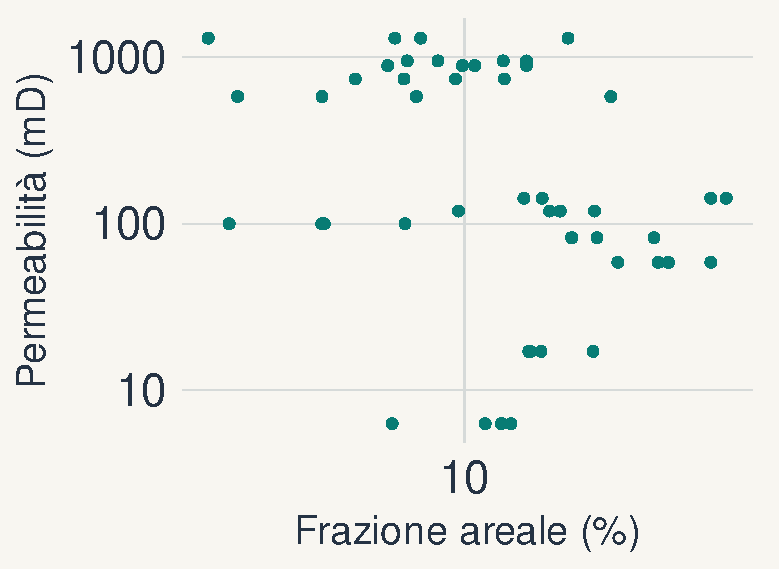
\includegraphics[width=\linewidth,height=6.15cm,keepaspectratio]{Figure/F01.pdf}\par}
\PSmall{Quarantotto sezioni su dodici carote. La permeabilità è in millidarcy e l’asse verticale è logaritmico.}
}};
\node[anchor=north west,inner sep=0] at([xshift=10.85cm,yshift=-2.12cm]current page.north west){\Colonna{8.16cm}{\PBody{Ogni punto rappresenta una sezione, mentre la permeabilità sull’asse verticale appartiene alla carota. Le sequenze orizzontali di quattro punti rendono visibile la risposta ripetuta e la variabilità dell’area fra immagini dello stesso campione. La scala logaritmica verticale permette di leggere permeabilità distribuite su più ordini di grandezza. Il grafico serve a riconoscere la struttura delle misure; un’analisi che utilizzasse quarantotto errori indipendenti per la risposta richiederebbe un’ipotesi incompatibile con tale struttura.}
}};
\end{tikzpicture}\end{frame}

\begin{frame}[plain]\hypertarget{slide10}{}
\bookmark[level=1,page=10]{Una sintesi areale per ogni carota}
\begin{tikzpicture}[remember picture,overlay]
\PilotChrome{Una sintesi areale per ogni carota}{VISUALIZZAZIONE E UNITÀ DI ANALISI}{10}{La sintesi esplicita l’unità del modello e conserva la provenienza dei valori aggregati.}
\node[anchor=north west,inner sep=0] at([xshift=.96cm,yshift=-2.12cm]current page.north west){\Colonna{9.40cm}{{\centering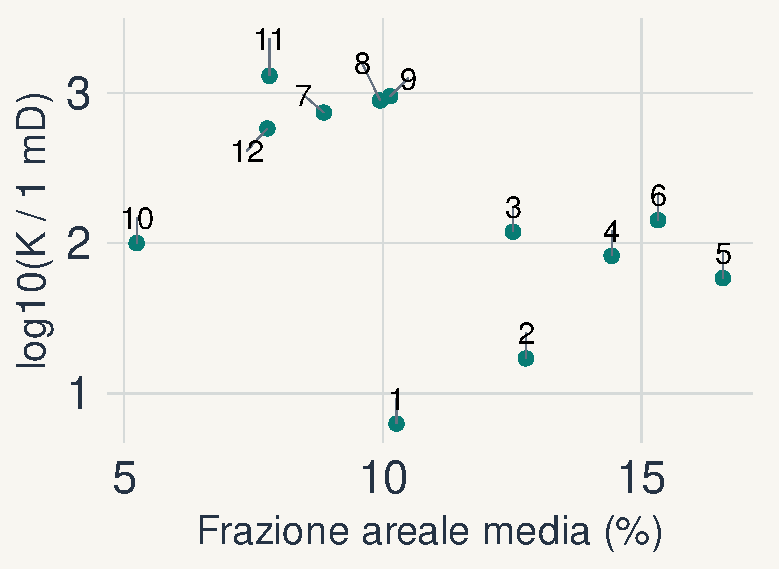
\includegraphics[width=\linewidth,height=6.15cm,keepaspectratio]{Figure/F02.pdf}\par}
\PSmall{$A_{ij}$: percentuale areale della sezione i nella carota j; $\bar A_j$: media delle quattro sezioni. Ordinata: $\log_{10}(K/1\,\mathrm{mD})$.}
}};
\node[anchor=north west,inner sep=0] at([xshift=10.85cm,yshift=-2.12cm]current page.north west){\Colonna{8.16cm}{\PBody{La media delle quattro frazioni areali rappresenta ciascuna carota attraverso un unico predittore, che viene associato alla sua permeabilità. Si ottengono dodici coppie, equiponderate nel modello successivo. La sintesi riduce la ripetizione della risposta, pur lasciando aperte l’incertezza della misura areale e la rappresentatività delle sezioni. I numeri accanto ai punti conservano gli identificativi ricostruiti e permettono di seguire i campioni nelle analisi di influenza, collegando il grafico alla tabella delle misure.}
\par\smallskip{\centering\adjustbox{max width=.98\linewidth}{$\displaystyle \overline A_j=\frac14\sum_{i=1}^{4}A_{ij},\qquad j=1,\ldots,12$}\par\smallskip}
}};
\end{tikzpicture}\end{frame}

\begin{frame}[plain]\hypertarget{slide11}{}
\bookmark[level=0,page=11]{Modello e interpretazione del parametro}
\bookmark[level=1,page=11]{Il modello definisce l’effetto da stimare}
\begin{tikzpicture}[remember picture,overlay]
\PilotChrome{Il modello definisce l’effetto da stimare}{MODELLO E INTERPRETAZIONE DEL PARAMETRO}{11}{La scala della risposta determina il significato fisico della pendenza e della trasformazione inversa.}
\node[anchor=north west,inner sep=0] at([xshift=.96cm,yshift=-2.12cm]current page.north west){\Colonna{9.40cm}{\PBody{La regressione collega il logaritmo decimale della permeabilità alla frazione areale media. La pendenza misura la variazione della risposta logaritmica per un punto percentuale di area, mentre la sua trasformazione in potenza di dieci esprime un fattore fra medie geometriche condizionate. La base del logaritmo e l’unità di riferimento devono essere dichiarate, poiché entrano nell’interpretazione dei coefficienti.}
\par\smallskip{\centering\adjustbox{max width=.98\linewidth}{$\displaystyle \begin{gathered}Y_j=\log_{10}\!\left(\frac{K_j}{1\ \mathrm{mD}}\right)=\alpha+\beta\overline A_j+\varepsilon_j\\\frac{G(K\mid A+1)}{G(K\mid A)}=10^\beta\end{gathered}$}\par\smallskip}
}};
\node[anchor=north west,inner sep=0] at([xshift=10.85cm,yshift=-2.12cm]current page.north west){\Colonna{8.16cm}{\PInfo{$K_j$: permeabilità della carota j; $\bar A_j$: percentuale areale media; $\alpha$: intercetta; $\beta$: pendenza. Si assume $E(\varepsilon_j\mid\bar A_j)=0$. G indica la media geometrica condizionata, definita tramite la media del logaritmo. La trasformazione inversa della retta non coincide in generale con la media aritmetica. L’associazione osservativa non identifica un effetto causale.}
}};
\end{tikzpicture}\end{frame}

\begin{frame}[plain]\hypertarget{slide12}{}
\bookmark[level=1,page=12]{Stima della pendenza attraverso la covariazione}
\begin{tikzpicture}[remember picture,overlay]
\PilotChrome{Stima della pendenza attraverso la covariazione}{MODELLO E INTERPRETAZIONE DEL PARAMETRO}{12}{Stima e interpretazione devono conservare scala, unità e dominio dell’associazione.}
\node[anchor=north west,inner sep=0] at([xshift=.96cm,yshift=-2.12cm]current page.north west){\Colonna{9.40cm}{{\centering\resizebox{0.90\linewidth}{!}{\begin{tikzpicture}[x=1cm,y=-.87cm,every node/.style={font=\fontsize{12.2}{15}\selectfont,text=Ink},arr/.style={-{Stealth[length=2mm]},line width=.8pt,draw=Classical}]\path[use as bounding box] (0,0) rectangle (7.45,6.2);
\draw[draw=Classical,fill=Classical!8,rounded corners=2pt,line width=.7pt] (0.5,0.8) rectangle (6.9,2.3);
\node[anchor=center,text=Ink,font=\fontsize{12.2}{15}\selectfont,text width=6cm,align=center] at (3.7,1.55) {Pendenza: $-0{,}08554$};
\draw[arr,draw=Quantum] (3.7,2.5)--(3.7,3.3);
\draw[draw=Quantum,fill=Quantum!8,rounded corners=2pt,line width=.7pt] (0.5,3.5) rectangle (6.9,5);
\node[anchor=center,text=Ink,font=\fontsize{12.2}{15}\selectfont,text width=6cm,align=center] at (3.7,4.25) {Fattore: $10^{\widehat\beta}=0{,}8212$};
\node[anchor=center,text=Ink,font=\fontsize{11}{15}\selectfont,text width=6.8cm,align=center] at (3.7,5.8) {Incremento di un punto percentuale areale};

\end{tikzpicture}}\par}
\PSmall{$\bar A_j$: area media della carota j; $Y_j=\log_{10}(K_j/1\,\mathrm{mD})$. $\bar A$ e $\bar Y$ sono le medie sulle dodici carote.}
}};
\node[anchor=north west,inner sep=0] at([xshift=10.85cm,yshift=-2.12cm]current page.north west){\Colonna{8.16cm}{\PBody{La stima ai minimi quadrati confronta la covariazione fra area e risposta logaritmica con la dispersione dell’area. Centrare entrambe le variabili rende esplicito che la pendenza descrive come i loro scostamenti si associno nel campione. Il codice verifica l’equivalenza fra la formula e il coefficiente restituito da lm. La stima ottenuta è circa meno 0,08554 per punto percentuale, mentre il fattore in scala originaria è circa 0,8212. Questi valori richiedono un intervallo e una diagnosi del modello prima dell’interpretazione conclusiva.}
\par\smallskip{\centering\adjustbox{max width=.98\linewidth}{$\displaystyle \widehat\beta=\frac{\sum_j(\overline A_j-\overline A)(Y_j-\overline Y)}{\sum_j(\overline A_j-\overline A)^2}$}\par\smallskip}
}};
\end{tikzpicture}\end{frame}

\begin{frame}[plain]\hypertarget{slide13}{}
\bookmark[level=1,page=13]{Adattamento e controllo numerico in R}
\begin{tikzpicture}[remember picture,overlay]
\PilotChrome{Adattamento e controllo numerico in R}{MODELLO E INTERPRETAZIONE DEL PARAMETRO}{13}{Il controllo numerico verifica il calcolo del modello; le sue assunzioni richiedono evidenza ulteriore.}
\node[anchor=north west,inner sep=0] at([xshift=.96cm,yshift=-2.12cm]current page.north west){\Colonna{9.40cm}{\PBody{Il frammento ricostruisce la sintesi per carota, trasforma la risposta e adatta la regressione. Il confronto con la formula della covarianza costituisce un controllo indipendente dell’implementazione del coefficiente. La tabella finale affianca stima ed errore standard, presi da summary, all’intervallo classico di confint, valido sotto le ipotesi del modello. Queste quantità vanno lette alla luce della struttura del campione: il completamento del comando non verifica le assunzioni.}
}};
\node[anchor=north west,inner sep=0] at([xshift=10.85cm,yshift=-2.12cm]current page.north west){\Colonna{8.16cm}{\begin{tcolorbox}[enhanced,arc=1.7mm,boxrule=.6pt,colback=white,colframe=Classical!60!Navy,colbacktitle=Navy,coltitle=white,fonttitle=\bfseries\small,title={R · calcolo riproducibile},left=1.7mm,right=1.3mm,top=1.1mm,bottom=1.1mm,before skip=1mm,after skip=1.0mm]\lstinputlisting[style=GeoR,language=R,basicstyle=\ttfamily\fontsize{8.6}{11.4}\selectfont]{Codice/modello.R}\end{tcolorbox}
\PLabel{Risultato in R}
\begin{tcolorbox}[colback=GeoTint,colframe=Rule,boxrule=.5pt,arc=1.4mm,left=2mm,right=1mm,top=1mm,bottom=1mm]{\fontsize{8.4}{10.9}\selectfont\ttfamily \mbox{\ \ \ \ \ \ \ \ \ \ \ \ Estimate\ Std.\ Error\ \ \ 2.5\ \%\ 97.5\ \%}\\\mbox{(Intercept)\ \ \ 3.1563\ \ \ \ \ 0.7196\ \ 1.5530\ 4.7595}\\\mbox{A\ \ \ \ \ \ \ \ \ \ \ \ -0.0855\ \ \ \ \ 0.0629\ -0.2257\ 0.0546}}\end{tcolorbox}
}};
\end{tikzpicture}\end{frame}

\begin{frame}[plain]\hypertarget{slide14}{}
\bookmark[level=1,page=14]{Intervallo classico e gradi di libertà}
\begin{tikzpicture}[remember picture,overlay]
\PilotChrome{Intervallo classico e gradi di libertà}{MODELLO E INTERPRETAZIONE DEL PARAMETRO}{14}{Un intervallo acquista significato attraverso il modello probabilistico che ne giustifica la costruzione.}
\node[anchor=north west,inner sep=0] at([xshift=.96cm,yshift=-2.12cm]current page.north west){\Colonna{9.40cm}{\PBody{Con dodici carote e due coefficienti stimati, la varianza residua utilizza dieci gradi di libertà. L’intervallo t per la pendenza assume errori indipendenti, gaussiani e con varianza costante attorno a una relazione lineare correttamente specificata. Nel campione l’errore standard è circa 0,06288 e l’intervallo al 95\% si estende da meno 0,22565 a più 0,05458. La presenza dello zero segnala la compatibilità di pendenze differenti con queste assunzioni e con l’informazione osservata.}
\par\smallskip{\centering\adjustbox{max width=.98\linewidth}{$\displaystyle \begin{gathered}\widehat\sigma^2=\frac{\sum_j\widehat\varepsilon_j^2}{12-2},\qquad SE(\widehat\beta)=\sqrt{\frac{\widehat\sigma^2}{\sum_j(\overline A_j-\overline A)^2}}\\IC_{95\%}=\widehat\beta\pm t_{0{,}975;10}SE(\widehat\beta)\end{gathered}$}\par\smallskip}
}};
\node[anchor=north west,inner sep=0] at([xshift=10.85cm,yshift=-2.12cm]current page.north west){\Colonna{8.16cm}{\PInfo{$\hat\varepsilon_j=Y_j-\hat Y_j$: residuo logaritmico; $\bar A_j$: percentuale areale della carota; $\bar A$: media delle dodici carote. SE indica l’errore standard; $t_{0,975;10}\simeq2,228$ è il quantile t. L’esattezza in piccolo campione dipende dalle ipotesi sugli errori; selezione delle carote e incertezza del predittore richiedono valutazioni ulteriori.}
}};
\end{tikzpicture}\end{frame}

\begin{frame}[plain]\hypertarget{slide15}{}
\bookmark[level=1,page=15]{Retta e incertezza della risposta media}
\begin{tikzpicture}[remember picture,overlay]
\PilotChrome{Retta e incertezza della risposta media}{MODELLO E INTERPRETAZIONE DEL PARAMETRO}{15}{L’incertezza della media stimata e quella di una nuova osservazione corrispondono a quantità diverse.}
\node[anchor=north west,inner sep=0] at([xshift=.96cm,yshift=-2.12cm]current page.north west){\Colonna{9.40cm}{{\centering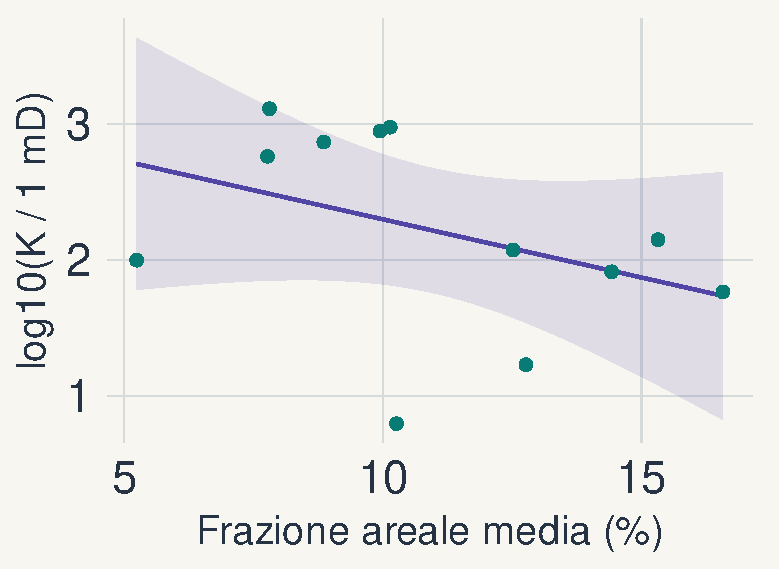
\includegraphics[width=\linewidth,height=6.15cm,keepaspectratio]{Figure/F03.pdf}\par}
\PSmall{Retta OLS e intervallo puntuale della media in scala log10. I dodici punti conservano il livello della carota.}
}};
\node[anchor=north west,inner sep=0] at([xshift=10.85cm,yshift=-2.12cm]current page.north west){\Colonna{8.16cm}{\PBody{La fascia attorno alla retta rappresenta l’intervallo puntuale al 95\% della media della risposta logaritmica, calcolato secondo il modello classico. La larghezza aumenta allontanandosi dall’area media del campione, perché diminuisce l’informazione disponibile sulla posizione della retta. Una previsione per una nuova carota richiederebbe anche la variabilità residua individuale e produrrebbe un intervallo più ampio. La figura mantiene il dominio delle aree osservate, evitando di attribuire alla relazione una validità esterna non verificata.}
}};
\end{tikzpicture}\end{frame}

\begin{frame}[plain]\hypertarget{slide16}{}
\bookmark[level=0,page=16]{Ricampionamento e sensibilità}
\bookmark[level=1,page=16]{Il bootstrap ricampiona intere carote}
\begin{tikzpicture}[remember picture,overlay]
\PilotChrome{Il bootstrap ricampiona intere carote}{RICAMPIONAMENTO E SENSIBILITÀ}{16}{La scelta dell’unità ricampionata conserva la struttura sulla quale si fonda l’inferenza.}
\node[anchor=north west,inner sep=0] at([xshift=.96cm,yshift=-2.12cm]current page.north west){\Colonna{9.40cm}{{\centering\resizebox{0.90\linewidth}{!}{\begin{tikzpicture}[x=1cm,y=-.87cm,every node/.style={font=\fontsize{12.2}{15}\selectfont,text=Ink},arr/.style={-{Stealth[length=2mm]},line width=.8pt,draw=Classical}]\path[use as bounding box] (0,0) rectangle (7.45,6.2);
\draw[draw=Classical,fill=Classical!8,rounded corners=2pt,line width=.7pt] (0.5,0.5) rectangle (6.9,1.8);
\node[anchor=center,text=Ink,font=\fontsize{12.2}{15}\selectfont,text width=6cm,align=center] at (3.7,1.15) {Dodici coppie a livello di carota};
\draw[arr,draw=Classical] (3.7,2)--(3.7,2.6);
\draw[draw=Quantum,fill=Quantum!8,rounded corners=2pt,line width=.7pt] (0.5,2.8) rectangle (6.9,4.1);
\node[anchor=center,text=Ink,font=\fontsize{11.5}{15}\selectfont,text width=6cm,align=center] at (3.7,3.45) {Estrazione con reinserimento e nuova retta};
\draw[arr,draw=Classical] (3.7,4.3)--(3.7,4.9);
\node[anchor=center,text=Ink,font=\fontsize{13}{15}\selectfont,text width=6.7cm,align=center] at (3.7,5.5) {Ripetizione: $\widehat\beta^{*(1)},\ldots,\widehat\beta^{*(4000)}$};

\end{tikzpicture}}\par}
}};
\node[anchor=north west,inner sep=0] at([xshift=10.85cm,yshift=-2.12cm]current page.north west){\Colonna{8.16cm}{\PBody{Ogni replica estrae dodici carote con reinserimento e ristima la pendenza sulle coppie area–permeabilità selezionate. Le quattro sezioni sono già rappresentate dalla media della rispettiva carota, per cui il ricampionamento mantiene l’unità della risposta. Il progetto conserva quattromila piani di estrazione condivisi, che rendono confrontabili le implementazioni indipendentemente dai generatori casuali. Con dodici unità osservate, la distribuzione bootstrap esplora la sensibilità alle molteplicità del campione disponibile e richiede cautela nelle conclusioni sulla coda.}
}};
\end{tikzpicture}\end{frame}

\begin{frame}[plain]\hypertarget{slide17}{}
\bookmark[level=1,page=17]{Distribuzione bootstrap della pendenza}
\begin{tikzpicture}[remember picture,overlay]
\PilotChrome{Distribuzione bootstrap della pendenza}{RICAMPIONAMENTO E SENSIBILITÀ}{17}{Il numero di ricampionamenti controlla la simulazione della procedura e lascia invariata l’informazione osservativa.}
\node[anchor=north west,inner sep=0] at([xshift=.96cm,yshift=-2.12cm]current page.north west){\Colonna{9.40cm}{{\centering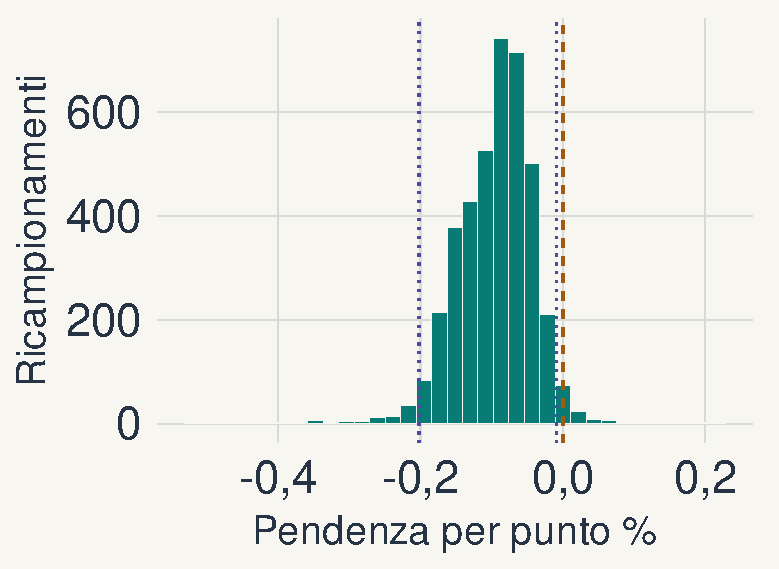
\includegraphics[width=\linewidth,height=6.15cm,keepaspectratio]{Figure/F04.pdf}\par}
\PSmall{$\hat\beta^*$: pendenza ricampionata; $Q_p$: quantile empirico. 4000 repliche; viola: estremi percentili; ocra: zero.}
}};
\node[anchor=north west,inner sep=0] at([xshift=10.85cm,yshift=-2.12cm]current page.north west){\Colonna{8.16cm}{\PBody{Le quattromila stime mostrano la variabilità prodotta dalle diverse molteplicità delle carote estratte. L’intervallo percentile utilizza i quantili al 2,5\% e 97,5\%, che in questa esecuzione valgono circa meno 0,20194 e meno 0,00893. Entrambi gli estremi risultano negativi, diversamente dall’intervallo t. La distribuzione riflette il campione disponibile e la procedura di ricampionamento; il numero elevato di repliche riduce l’errore Monte Carlo, senza aumentare il numero di carote osservate.}
\par\smallskip{\centering\adjustbox{max width=.98\linewidth}{$\displaystyle IC_{perc}=\left[Q_{0{,}025}(\widehat\beta^*),Q_{0{,}975}(\widehat\beta^*)\right]$}\par\smallskip}
}};
\end{tikzpicture}\end{frame}

\begin{frame}[plain]\hypertarget{slide18}{}
\bookmark[level=1,page=18]{Confrontare intervalli costruiti diversamente}
\begin{tikzpicture}[remember picture,overlay]
\PilotChrome{Confrontare intervalli costruiti diversamente}{RICAMPIONAMENTO E SENSIBILITÀ}{18}{La discordanza fra procedure orienta l’esame delle assunzioni e la richiesta di nuove evidenze.}
\node[anchor=north west,inner sep=0] at([xshift=.96cm,yshift=-2.12cm]current page.north west){\Colonna{9.40cm}{{\centering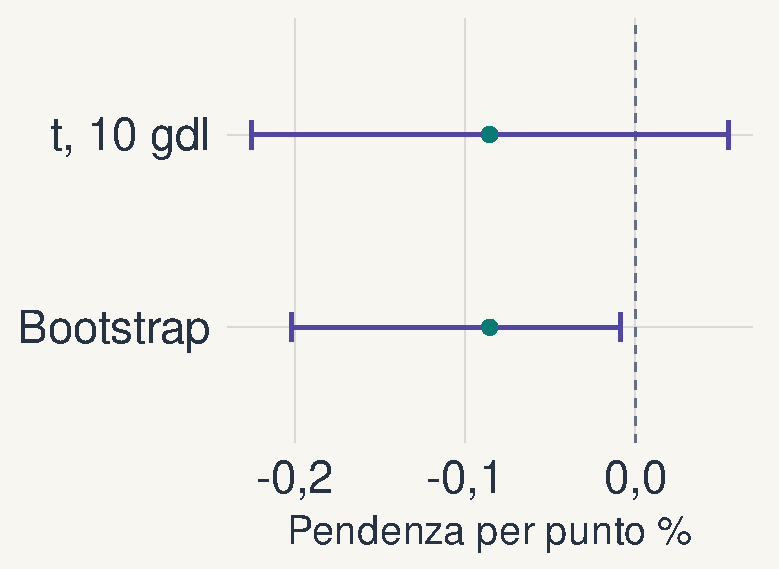
\includegraphics[width=\linewidth,height=6.15cm,keepaspectratio]{Figure/F07.pdf}\par}
\PSmall{Stessa stima puntuale, intervallo t e intervallo percentile. Il riferimento verticale indica la pendenza nulla.}
}};
\node[anchor=north west,inner sep=0] at([xshift=10.85cm,yshift=-2.12cm]current page.north west){\Colonna{8.16cm}{\PBody{L’intervallo classico comprende lo zero, mentre quello percentile resta interamente negativo. Il disaccordo rende visibile la dipendenza della conclusione da assunzioni e approssimazioni, particolarmente rilevante con dodici carote. L’analisi riporta entrambe le costruzioni e ne discute le condizioni, senza scegliere quella che produce l’esito più favorevole. Il test classico della pendenza nulla restituisce un p-value di circa 0,204, mentre il coefficiente di determinazione è circa 0,156: queste quantità descrivono aspetti differenti del modello e non eliminano il problema della limitata informazione.}
}};
\end{tikzpicture}\end{frame}

\begin{frame}[plain]\hypertarget{slide19}{}
\bookmark[level=1,page=19]{Residui e forma della relazione}
\begin{tikzpicture}[remember picture,overlay]
\PilotChrome{Residui e forma della relazione}{RICAMPIONAMENTO E SENSIBILITÀ}{19}{Le proprietà algebriche dell’adattamento devono essere distinte dalle ipotesi probabilistiche sugli errori.}
\node[anchor=north west,inner sep=0] at([xshift=.96cm,yshift=-2.12cm]current page.north west){\Colonna{9.40cm}{{\centering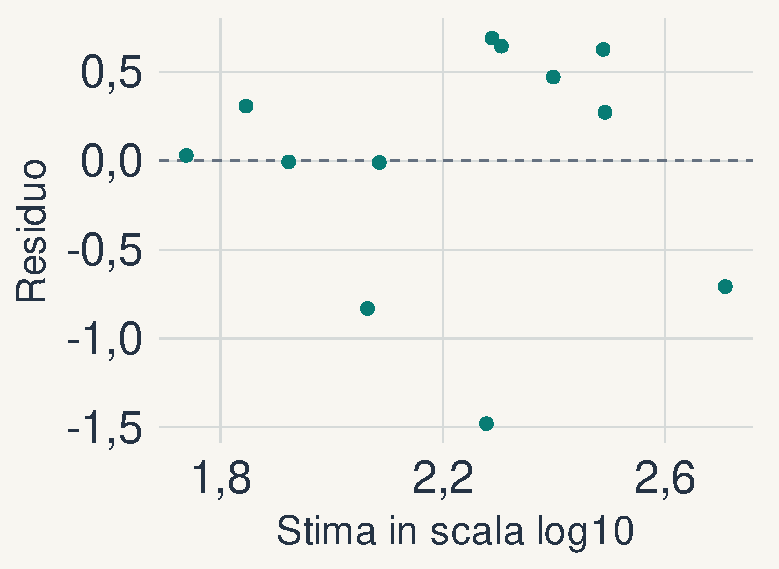
\includegraphics[width=\linewidth,height=6.15cm,keepaspectratio]{Figure/F05.pdf}\par}
\PSmall{X: matrice con colonne 1 e percentuale areale media; $\hat\varepsilon$: vettore dei dodici residui. La linea orizzontale indica zero.}
}};
\node[anchor=north west,inner sep=0] at([xshift=10.85cm,yshift=-2.12cm]current page.north west){\Colonna{8.16cm}{\PBody{I residui descrivono gli scostamenti delle risposte dalla retta adattata e vengono esaminati rispetto ai valori stimati. Curvature, variazioni di dispersione o punti isolati possono suggerire limiti della specificazione, benché dodici osservazioni offrano una capacità diagnostica ridotta. L’assenza di un andamento evidente nel grafico lascia quindi aperta l’adeguatezza delle assunzioni. I residui OLS sono ortogonali alle colonne della matrice del modello per costruzione; questa proprietà verifica il calcolo e non costituisce una prova dell’indipendenza degli errori geologici.}
\par\smallskip{\centering\adjustbox{max width=.98\linewidth}{$\displaystyle X^\top\widehat\varepsilon=0$}\par\smallskip}
}};
\end{tikzpicture}\end{frame}

\begin{frame}[plain]\hypertarget{slide20}{}
\bookmark[level=1,page=20]{Escludere una carota alla volta come diagnosi}
\begin{tikzpicture}[remember picture,overlay]
\PilotChrome{Escludere una carota alla volta come diagnosi}{RICAMPIONAMENTO E SENSIBILITÀ}{20}{L’influenza di un’osservazione richiede esame e documentazione prima di una decisione di esclusione.}
\node[anchor=north west,inner sep=0] at([xshift=.96cm,yshift=-2.12cm]current page.north west){\Colonna{9.40cm}{{\centering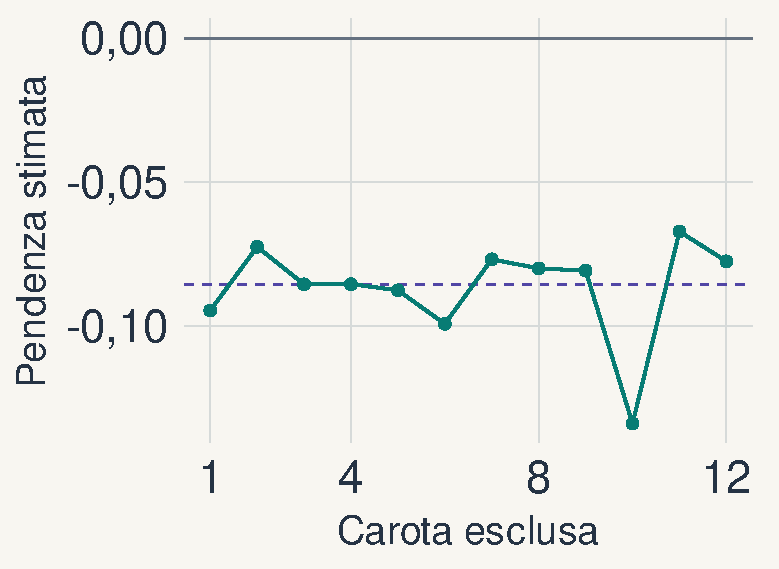
\includegraphics[width=\linewidth,height=6.15cm,keepaspectratio]{Figure/F06.pdf}\par}
\PSmall{$\bar A_i$: percentuale areale; $Y_i=\log_{10}(K_i/1\,\mathrm{mD})$. Si omette la carota j. Viola: pendenza su tutte le dodici.}
}};
\node[anchor=north west,inner sep=0] at([xshift=10.85cm,yshift=-2.12cm]current page.north west){\Colonna{8.16cm}{\PBody{La regressione viene ripetuta dodici volte, omettendo a turno una carota e mantenendo invariati modello e trasformazione. Le pendenze risultano comprese fra circa meno 0,13372 e meno 0,06707, mostrando una variazione della grandezza dell’associazione senza inversione del segno. La procedura identifica il contributo dei singoli campioni alla stima e orienta il controllo delle misure. L’esclusione definitiva richiederebbe una motivazione indipendente dalla convenienza del risultato e dovrebbe essere documentata insieme all’analisi sul campione completo.}
\par\smallskip{\centering\adjustbox{max width=.98\linewidth}{$\displaystyle (\hat\alpha_{(-j)},\hat\beta_{(-j)})=\arg\min_{a,b}\sum_{i\ne j}(Y_i-a-b\bar A_i)^2$}\par\smallskip}
}};
\end{tikzpicture}\end{frame}

\begin{frame}[plain]\hypertarget{slide21}{}
\bookmark[level=0,page=21]{Argomentazione geologica e consegna}
\bookmark[level=1,page=21]{Un segno inatteso richiede una spiegazione fondata}
\begin{tikzpicture}[remember picture,overlay]
\PilotChrome{Un segno inatteso richiede una spiegazione fondata}{ARGOMENTAZIONE GEOLOGICA E CONSEGNA}{21}{L’interpretazione fisica deve rispettare la proprietà effettivamente misurata e il dominio del campione.}
\node[anchor=north west,inner sep=0] at([xshift=.96cm,yshift=-2.12cm]current page.north west){\Colonna{9.40cm}{{\centering\resizebox{0.90\linewidth}{!}{\begin{tikzpicture}[x=1cm,y=-.87cm,every node/.style={font=\fontsize{12.2}{15}\selectfont,text=Ink},arr/.style={-{Stealth[length=2mm]},line width=.8pt,draw=Classical}]\path[use as bounding box] (0,0) rectangle (7.45,6.2);
\draw[draw=Classical,fill=Classical!8,rounded corners=2pt,line width=.7pt] (0.5,0.5) rectangle (6.9,1.8);
\node[anchor=center,text=Ink,font=\fontsize{12.2}{15}\selectfont,text width=6cm,align=center] at (3.7,1.15) {Evidenza: associazione nel campione};
\draw[arr,draw=Classical] (3.7,2)--(3.7,2.7);
\draw[draw=Quantum,fill=Quantum!8,rounded corners=2pt,line width=.7pt] (0.5,2.9) rectangle (6.9,4.2);
\node[anchor=center,text=Ink,font=\fontsize{11.5}{15}\selectfont,text width=6cm,align=center] at (3.7,3.55) {Meccanismo: geometria e connessione 3D};
\node[anchor=center,text=Ink,font=\fontsize{11.5}{15}\selectfont,text width=6.7cm,align=center] at (3.7,5.4) {Nuove misure collegano il proxy alla proprietà di trasporto.};

\end{tikzpicture}}\par}
}};
\node[anchor=north west,inner sep=0] at([xshift=10.85cm,yshift=-2.12cm]current page.north west){\Colonna{8.16cm}{\PBody{La pendenza negativa osservata non autorizza a correggere il segno delle variabili o a concludere che una maggiore porosità riduca in generale la permeabilità. La frazione areale misura una proprietà delle sezioni, mentre trasporto, connessione dei pori, tortuosità e dimensione delle gole appartengono a una struttura tridimensionale più articolata. Il campione storico e il modello lineare rappresentano ulteriori limiti. La conclusione sostiene dunque l’associazione descritta nelle carote disponibili, accompagnandola con l’incertezza e con le misure che servirebbero a esaminarne il meccanismo.}
}};
\end{tikzpicture}\end{frame}

\begin{frame}[plain]\hypertarget{slide22}{}
\bookmark[level=1,page=22]{Relazione, esercizio e criteri di discussione}
\begin{tikzpicture}[remember picture,overlay]
\PilotChrome{Relazione, esercizio e criteri di discussione}{ARGOMENTAZIONE GEOLOGICA E CONSEGNA}{22}{La consegna deve rendere verificabili il calcolo e il percorso che conduce dall’evidenza alla conclusione.}
\node[anchor=north west,inner sep=0] at([xshift=.96cm,yshift=-2.12cm]current page.north west){\Colonna{9.40cm}{\PBody{La relazione presenta provenienza, ricostruzione delle carote, trasformazione areale, modello, stima con unità, intervalli e diagnostica. L’esercizio richiede due figure motivate, il confronto fra intervallo t e bootstrap e una discussione della sensibilità alle singole carote. Una risposta adeguata collega il disaccordo inferenziale al piccolo campione e alle assunzioni, evitando di ridurlo alla scelta di una soglia di significatività. L’estensione facoltativa esamina un predittore alternativo soltanto dopo averne verificato definizione e disponibilità nei dati originali.}
}};
\node[anchor=north west,inner sep=0] at([xshift=10.85cm,yshift=-2.12cm]current page.north west){\Colonna{8.16cm}{\PInfo{Lo script R/P01\_figure.R ricostruisce calcoli, tabelle e grafici dalla cartella dati/progetti. Le verifiche controllano gruppi, dominio, corrispondenza con rock, stima della pendenza e piano bootstrap. Il progetto raccorda misura e campionamento, inferenza e regressione, sviluppati nei moduli M01, M05 e M07.}
}};
\end{tikzpicture}\end{frame}

\begin{frame}[plain]\hypertarget{slide23}{}
\bookmark[level=0,page=23]{Laboratori della spedizione}
\bookmark[level=1,page=23]{Tre fasi della spedizione nel laboratorio}
\begin{tikzpicture}[remember picture,overlay]
\PilotChrome{Tre fasi della spedizione nel laboratorio}{LABORATORI DELLA SPEDIZIONE}{23}{Gli esperimenti usano dati sintetici; la conclusione sul caso resta quella ottenuta dalle dodici carote.}
\node[anchor=north west,inner sep=0] at([xshift=.96cm,yshift=-2.12cm]current page.north west){\Colonna{9.40cm}{{\centering\resizebox{0.97\linewidth}{!}{\begin{tikzpicture}[x=1cm,y=1cm,every node/.style={font=\sffamily\fontsize{9.2}{11}\selectfont,text=Ink}]
\node[draw=Classical,fill=Classical,rounded corners=2mm,text=white,text width=2.45cm,align=flush center,minimum height=1.55cm,anchor=west,font=\sffamily\bfseries\fontsize{9.2}{11}\selectfont] (f0) at (0,0.00) {1. Definire l’unità};
\node[draw=Classical!60,fill=Classical!6,rounded corners=1.5mm,line width=.6pt,text width=2.8cm,align=flush center,minimum height=1.55cm,anchor=west] (e00) at (2.95,0.00) {Definire la quantità di interesse\\[1pt]{\fontsize{7.6}{9}\selectfont\color{Muted}m01-estimando}};
\node[draw=Rule,fill=white,rounded corners=1.5mm,line width=.6pt,text width=2.8cm,align=flush center,minimum height=1.55cm,anchor=west] (e01) at (6.10,0.00) {Misure replicate e unità indipendenti\\[1pt]{\fontsize{7.6}{9}\selectfont\color{Muted}m01-gerarchia}};
\draw[pEdge] (f0.east)--(e00.west);
\node[draw=Classical,fill=Classical,rounded corners=2mm,text=white,text width=2.45cm,align=flush center,minimum height=1.55cm,anchor=west,font=\sffamily\bfseries\fontsize{9.2}{11}\selectfont] (f1) at (0,-1.95) {2. Esaminare la relazione};
\draw[pEdge] (f0.south)--(f1.north);
\node[draw=Classical!60,fill=Classical!6,rounded corners=1.5mm,line width=.6pt,text width=2.8cm,align=flush center,minimum height=1.55cm,anchor=west] (e10) at (2.95,-1.95) {Scale lineari e logaritmiche\\[1pt]{\fontsize{7.6}{9}\selectfont\color{Muted}m03-scale}};
\node[draw=Rule,fill=white,rounded corners=1.5mm,line width=.6pt,text width=2.8cm,align=flush center,minimum height=1.55cm,anchor=west] (e11) at (6.10,-1.95) {La geometria dei minimi quadrati\\[1pt]{\fontsize{7.6}{9}\selectfont\color{Muted}m07-minimi-quadrati}};
\draw[pEdge] (f1.east)--(e10.west);
\node[draw=Classical,fill=Classical,rounded corners=2mm,text=white,text width=2.45cm,align=flush center,minimum height=1.55cm,anchor=west,font=\sffamily\bfseries\fontsize{9.2}{11}\selectfont] (f2) at (0,-3.90) {3. Valutare la stabilità};
\draw[pEdge] (f1.south)--(f2.north);
\node[draw=Classical!60,fill=Classical!6,rounded corners=1.5mm,line width=.6pt,text width=2.8cm,align=flush center,minimum height=1.55cm,anchor=west] (e20) at (2.95,-3.90) {Leva e influenza di un’osservazione\\[1pt]{\fontsize{7.6}{9}\selectfont\color{Muted}m07-influenza}};
\node[draw=Rule,fill=white,rounded corners=1.5mm,line width=.6pt,text width=2.8cm,align=flush center,minimum height=1.55cm,anchor=west] (e21) at (6.10,-3.90) {Ricampionamento per stazioni\\[1pt]{\fontsize{7.6}{9}\selectfont\color{Muted}m05-ricampionamento}};
\draw[pEdge] (f2.east)--(e20.west);
\end{tikzpicture}
}\par}
\PSmall{Fasi della spedizione. Il primo esperimento di ogni fase ha le pagine Scenario A e Confronto.}
}};
\node[anchor=north west,inner sep=0] at([xshift=10.85cm,yshift=-2.12cm]current page.north west){\Colonna{8.16cm}{\PBody{Gli esperimenti ripetono su dati sintetici tre scelte della spedizione: l’unità da sintetizzare, la scala della relazione, il peso di una singola osservazione. Ogni fase ha uno scenario di partenza e un confronto con un solo parametro modificato.}
\vspace{.2cm}\PLabel{Altri esperimenti delle fasi}
\PLab{https://marzione00.github.io/Lab_Geo/\#laboratorio/m01-gerarchia}{Misure replicate e unità indipendenti · m01-gerarchia}
\PLab{https://marzione00.github.io/Lab_Geo/\#laboratorio/m07-minimi-quadrati}{La geometria dei minimi quadrati · m07-minimi-quadrati}
\PLab{https://marzione00.github.io/Lab_Geo/\#laboratorio/m05-ricampionamento}{Ricampionamento per stazioni · m05-ricampionamento}
}};
\end{tikzpicture}\end{frame}

\begin{frame}[plain]\hypertarget{slide24}{}
\bookmark[level=1,page=24]{Definire la quantità di interesse}
\begin{tikzpicture}[remember picture,overlay]
\PilotChrome{Definire la quantità di interesse}{LABORATORI DELLA SPEDIZIONE}{24}{Distinguere media delle misure e media delle unità geologiche.}
\node[anchor=north west,inner sep=0] at([xshift=.96cm,yshift=-2.12cm]current page.north west){\Colonna{9.40cm}{{\centering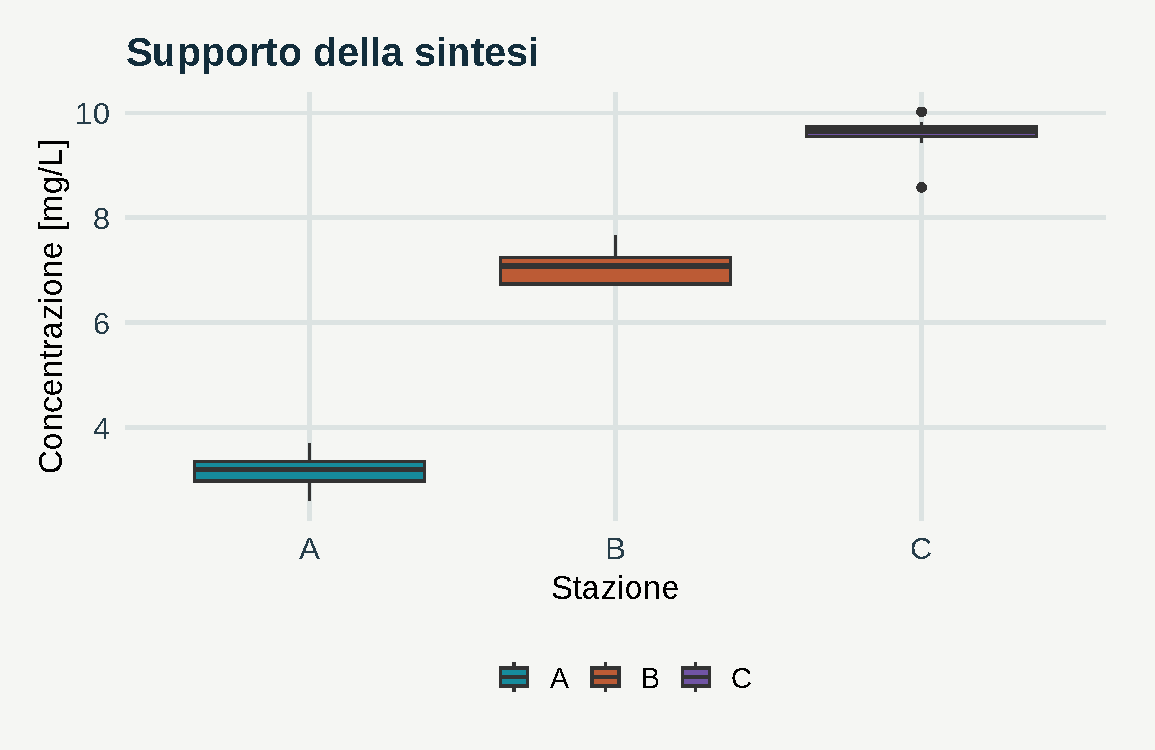
\includegraphics[width=\linewidth,height=6.0cm,keepaspectratio]{Esperimenti/m01-estimando-A.pdf}\par}
\PSmall{Misure nella stazione A: 20. Seme: 17.}
}};
\node[anchor=north west,inner sep=0] at([xshift=10.85cm,yshift=-2.12cm]current page.north west){\Colonna{8.16cm}{\PLabel{Scenario A · simulazione}
\PBody{Le stazioni rappresentano unità geologiche con concentrazioni medie differenti. Aumentando il numero di misure nella prima stazione, cresce il suo peso nella media complessiva delle osservazioni, mentre la media delle medie assegna lo stesso peso a ciascuna stazione, indipendentemente dall’intensità della raccolta.}
\par\smallskip{\centering\adjustbox{max width=.98\linewidth}{$\displaystyle \bar x_{\rm misure}=\frac{\sum_g n_g\bar x_g}{\sum_g n_g},\quad \bar x_{\rm stazioni}=G^{-1}\sum_g\bar x_g$}\par\smallskip}
\PSmall{$g$ identifica la stazione; $n_g$ ne indica la numerosità; $\bar x_g$ è la sua media campionaria; $G$ è il numero delle stazioni.}
}};
\node[anchor=north east,inner sep=0] at([xshift=17.1cm,yshift=-12.04cm]current page.north west){\fontsize{7.7}{9}\selectfont \href{https://marzione00.github.io/Lab_Geo/\#laboratorio/m01-estimando}{\color{Classical}\bfseries Apri il laboratorio · m01-estimando}};
\end{tikzpicture}\end{frame}

\begin{frame}[plain]\hypertarget{slide25}{}
\bookmark[level=1,page=25]{Confronto | Definire la quantità di interesse}
\begin{tikzpicture}[remember picture,overlay]
\PilotChrome{Confronto | Definire la quantità di interesse}{LABORATORI DELLA SPEDIZIONE}{25}{Il peso attribuito a ogni unità determina la quantità sintetizzata.}
\node[anchor=north west,inner sep=0] at([xshift=.96cm,yshift=-2.12cm]current page.north west){\Colonna{9.40cm}{{\centering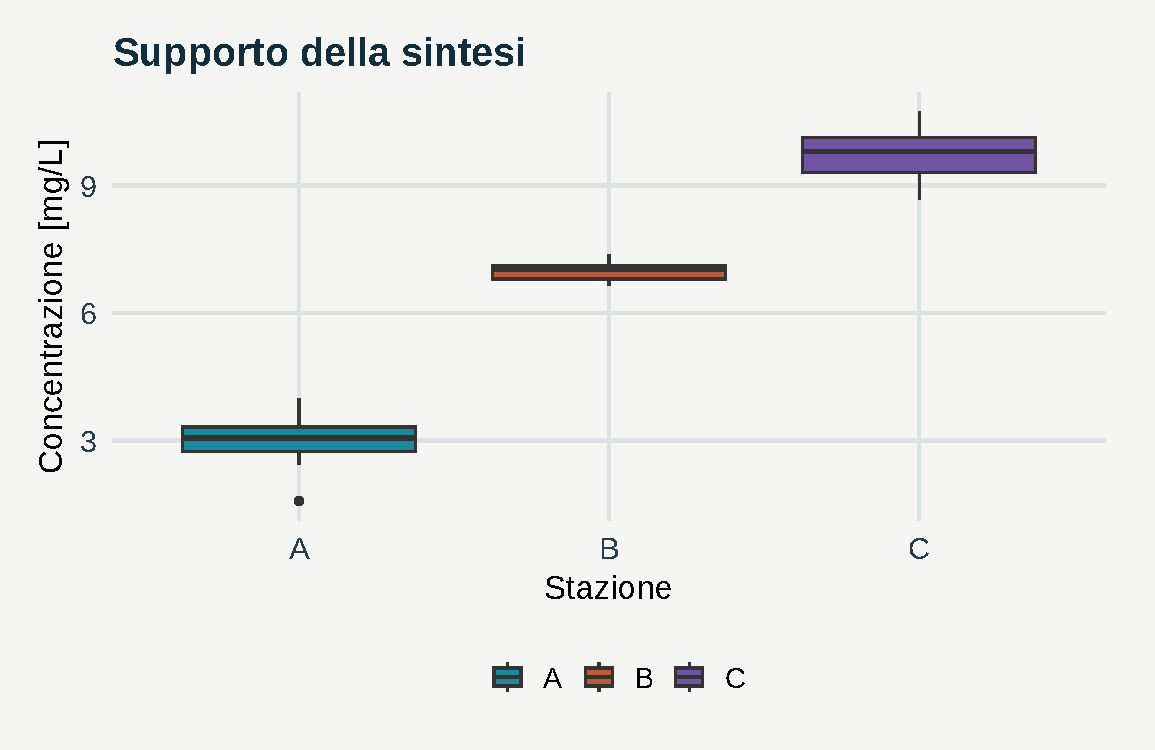
\includegraphics[width=\linewidth,height=5.6cm,keepaspectratio]{Esperimenti/m01-estimando-B.pdf}\par}
\PSmall{Misure nella stazione A: 20 $\to$ 60. Tutti gli altri parametri e il seme sono fissi.}
}};
\node[anchor=north west,inner sep=0] at([xshift=10.85cm,yshift=-2.12cm]current page.north west){\Colonna{8.16cm}{\PLabel{Confronto fra gli scenari}
{\fontsize{10.2}{12.8}\selectfont\begin{tabular}{@{}>{\raggedright\arraybackslash}p{0.48\linewidth}@{\hspace{.13cm}}>{\raggedright\arraybackslash}p{0.224\linewidth}@{\hspace{.13cm}}>{\raggedright\arraybackslash}p{0.224\linewidth}@{}}\toprule Grandezza & A & B\\[2.3pt]
\midrule 
Media delle misure & 5,75 & 4,38\\[2.3pt]
Media delle stazioni & 6,61 & 6,59\\[2.3pt]
\bottomrule\end{tabular}\par}
\vspace{.25cm}\PBody{Con sessanta misure nella stazione A la media delle misure scende da 5,75 a 4,38 e si avvicina al livello della stazione più campionata, mentre la media delle stazioni resta prossima a 6,6. Soltanto la prima sintesi dipende dall’intensità della raccolta.}
}};
\node[anchor=north east,inner sep=0] at([xshift=17.1cm,yshift=-12.04cm]current page.north west){\fontsize{7.7}{9}\selectfont \href{https://marzione00.github.io/Lab_Geo/\#laboratorio/m01-estimando}{\color{Classical}\bfseries Apri il laboratorio · m01-estimando}};
\end{tikzpicture}\end{frame}

\begin{frame}[plain]\hypertarget{slide26}{}
\bookmark[level=1,page=26]{Scale lineari e logaritmiche}
\begin{tikzpicture}[remember picture,overlay]
\PilotChrome{Scale lineari e logaritmiche}{LABORATORI DELLA SPEDIZIONE}{26}{Esaminare un processo moltiplicativo su due scale.}
\node[anchor=north west,inner sep=0] at([xshift=.96cm,yshift=-2.12cm]current page.north west){\Colonna{9.40cm}{{\centering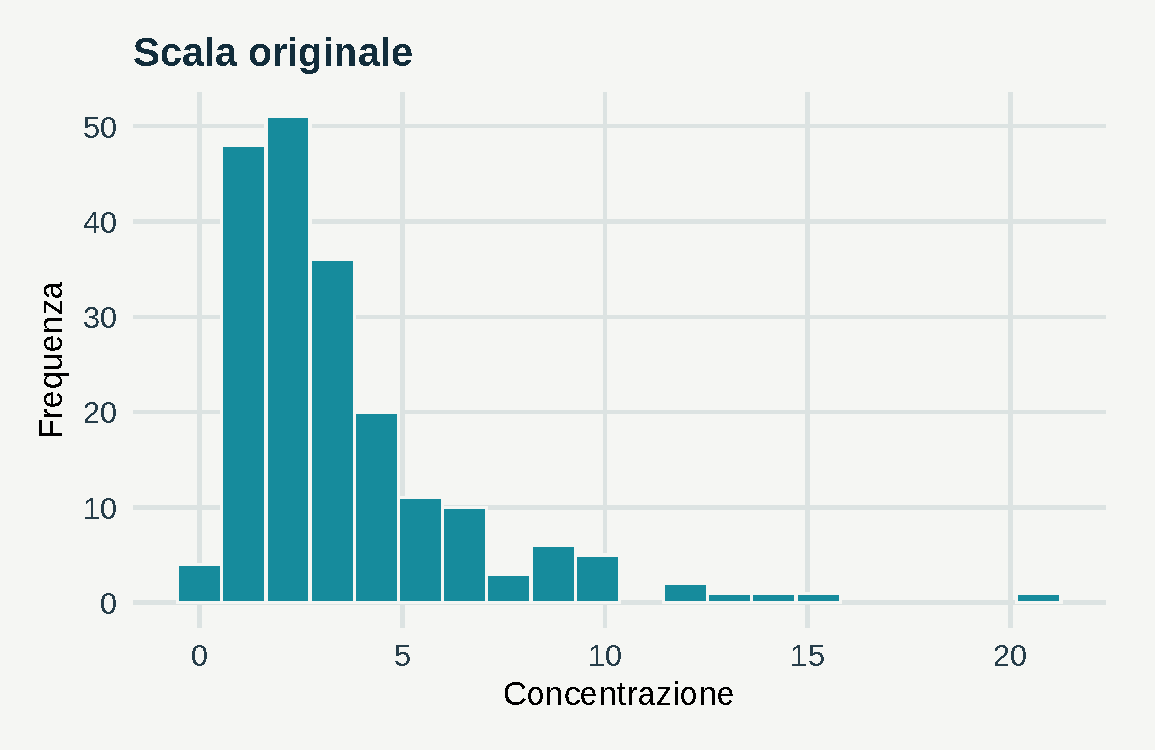
\includegraphics[width=\linewidth,height=6.0cm,keepaspectratio]{Esperimenti/m03-scale-A.pdf}\par}
\PSmall{Deviazione standard logaritmica: 0,7. Seme: 17.}
}};
\node[anchor=north west,inner sep=0] at([xshift=10.85cm,yshift=-2.12cm]current page.north west){\Colonna{8.16cm}{\PLabel{Scenario A · simulazione}
\PBody{Le concentrazioni simulate sono positive e seguono un modello lognormale. Il parametro modificabile è la deviazione standard dei logaritmi, che determina l’ampiezza della variabilità moltiplicativa e l’importanza della coda destra nella scala originale.}
\par\smallskip{\centering\adjustbox{max width=.98\linewidth}{$\displaystyle \log(xy)=\log x+\log y$}\par\smallskip}
\PSmall{$x$ e $y$ sono quantità positive; $\log$ è il logaritmo naturale. La media geometrica campionaria è $\exp(n^{-1}\sum_i\log x_i)$.}
}};
\node[anchor=north east,inner sep=0] at([xshift=17.1cm,yshift=-12.04cm]current page.north west){\fontsize{7.7}{9}\selectfont \href{https://marzione00.github.io/Lab_Geo/\#laboratorio/m03-scale}{\color{Classical}\bfseries Apri il laboratorio · m03-scale}};
\end{tikzpicture}\end{frame}

\begin{frame}[plain]\hypertarget{slide27}{}
\bookmark[level=1,page=27]{Confronto | Scale lineari e logaritmiche}
\begin{tikzpicture}[remember picture,overlay]
\PilotChrome{Confronto | Scale lineari e logaritmiche}{LABORATORI DELLA SPEDIZIONE}{27}{Il logaritmo trasforma rapporti in differenze e modifica la quantità sintetizzata.}
\node[anchor=north west,inner sep=0] at([xshift=.96cm,yshift=-2.12cm]current page.north west){\Colonna{9.40cm}{{\centering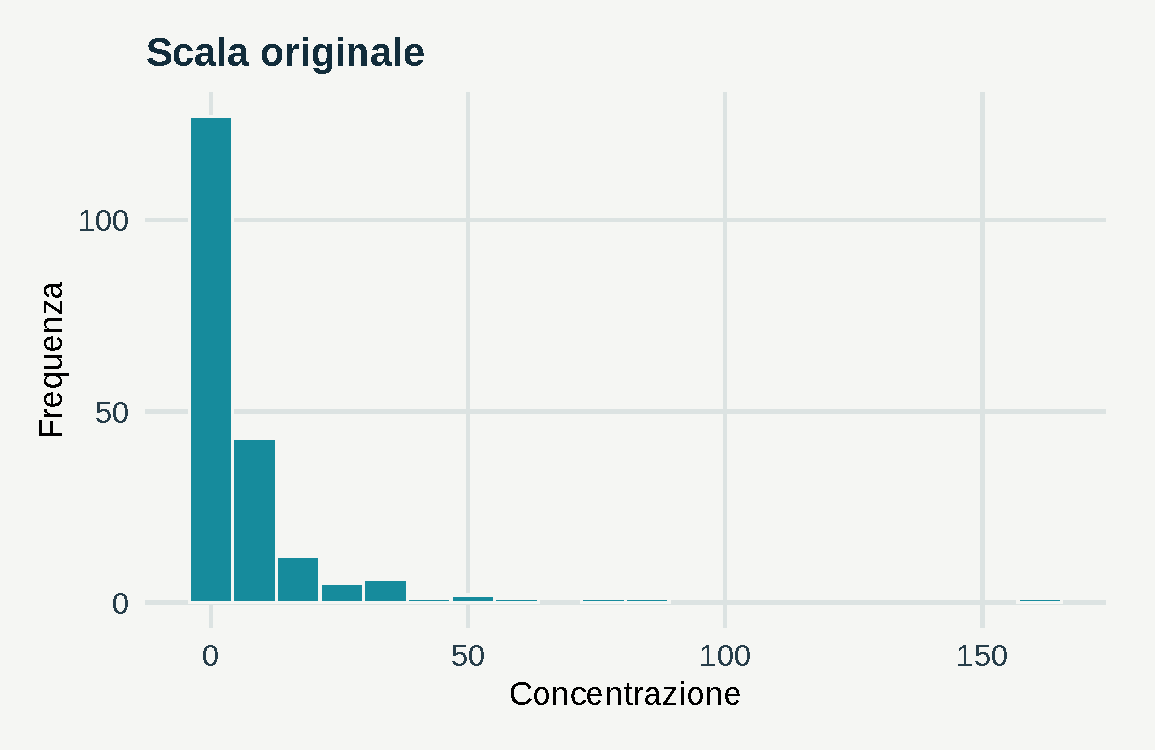
\includegraphics[width=\linewidth,height=5.6cm,keepaspectratio]{Esperimenti/m03-scale-B.pdf}\par}
\PSmall{Deviazione standard logaritmica: 0,7 $\to$ 1,4. Tutti gli altri parametri e il seme sono fissi.}
}};
\node[anchor=north west,inner sep=0] at([xshift=10.85cm,yshift=-2.12cm]current page.north west){\Colonna{8.16cm}{\PLabel{Confronto fra gli scenari}
{\fontsize{10.2}{12.8}\selectfont\begin{tabular}{@{}>{\raggedright\arraybackslash}p{0.48\linewidth}@{\hspace{.13cm}}>{\raggedright\arraybackslash}p{0.224\linewidth}@{\hspace{.13cm}}>{\raggedright\arraybackslash}p{0.224\linewidth}@{}}\toprule Grandezza & A & B\\[2.3pt]
\midrule 
Media aritmetica & 3,49 & 7,69\\[2.3pt]
Media geometrica & 2,62 & 2,52\\[2.3pt]
\bottomrule\end{tabular}\par}
\vspace{.25cm}\PBody{Con deviazione standard logaritmica 1,4 la media aritmetica sale da 3,49 a 7,69, trascinata dalla coda destra, mentre la media geometrica resta vicina a 2,5. Nella spedizione la scala logaritmica rende la pendenza un fattore fra medie geometriche della permeabilità.}
}};
\node[anchor=north east,inner sep=0] at([xshift=17.1cm,yshift=-12.04cm]current page.north west){\fontsize{7.7}{9}\selectfont \href{https://marzione00.github.io/Lab_Geo/\#laboratorio/m03-scale}{\color{Classical}\bfseries Apri il laboratorio · m03-scale}};
\end{tikzpicture}\end{frame}

\begin{frame}[plain]\hypertarget{slide28}{}
\bookmark[level=1,page=28]{Leva e influenza di un’osservazione}
\begin{tikzpicture}[remember picture,overlay]
\PilotChrome{Leva e influenza di un’osservazione}{LABORATORI DELLA SPEDIZIONE}{28}{Distinguere distanza nel predittore e influenza sul modello.}
\node[anchor=north west,inner sep=0] at([xshift=.96cm,yshift=-2.12cm]current page.north west){\Colonna{9.40cm}{{\centering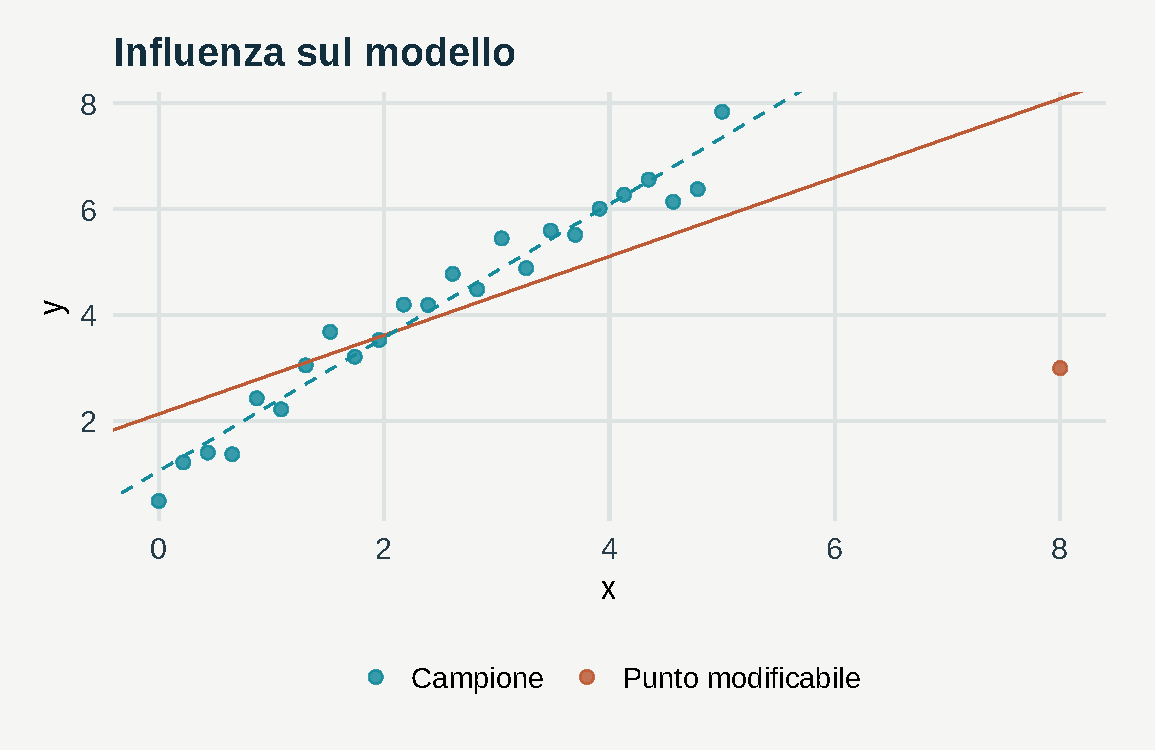
\includegraphics[width=\linewidth,height=5.0cm,keepaspectratio]{Esperimenti/m07-influenza-A.pdf}\par}
\PSmall{Coordinata X del punto: 8. Seme: 17.}
\PSmall{$D_i$ è la distanza di Cook del punto $i$; $e_i$ è il residuo; $h_{ii}$ è la leva. $\widehat\sigma^2$ è la varianza residua stimata e $p$ conta i coefficienti del modello, inclusa l’intercetta; qui $p=2$.}
}};
\node[anchor=north west,inner sep=0] at([xshift=10.85cm,yshift=-2.12cm]current page.north west){\Colonna{8.16cm}{\PLabel{Scenario A · simulazione}
\PBody{Il campione contiene una relazione lineare alla quale si aggiunge un’osservazione modificabile. Spostandone separatamente le coordinate, si possono distinguere una posizione insolita lungo il predittore e uno scostamento dalla relazione stimata. La leva dipende dalla geometria delle x; l’influenza considera anche il residuo e la variazione indotta sull’adattamento.}
\par\smallskip{\centering\adjustbox{max width=.98\linewidth}{$\displaystyle D_i=\frac{e_i^2}{p\widehat\sigma^2}\frac{h_{ii}}{(1-h_{ii})^2}$}\par\smallskip}
}};
\node[anchor=north east,inner sep=0] at([xshift=17.1cm,yshift=-12.04cm]current page.north west){\fontsize{7.7}{9}\selectfont \href{https://marzione00.github.io/Lab_Geo/\#laboratorio/m07-influenza}{\color{Classical}\bfseries Apri il laboratorio · m07-influenza}};
\end{tikzpicture}\end{frame}

\begin{frame}[plain]\hypertarget{slide29}{}
\bookmark[level=1,page=29]{Confronto | Leva e influenza di un’osservazione}
\begin{tikzpicture}[remember picture,overlay]
\PilotChrome{Confronto | Leva e influenza di un’osservazione}{LABORATORI DELLA SPEDIZIONE}{29}{L’influenza combina geometria del predittore e scostamento dalla relazione stimata.}
\node[anchor=north west,inner sep=0] at([xshift=.96cm,yshift=-2.12cm]current page.north west){\Colonna{9.40cm}{{\centering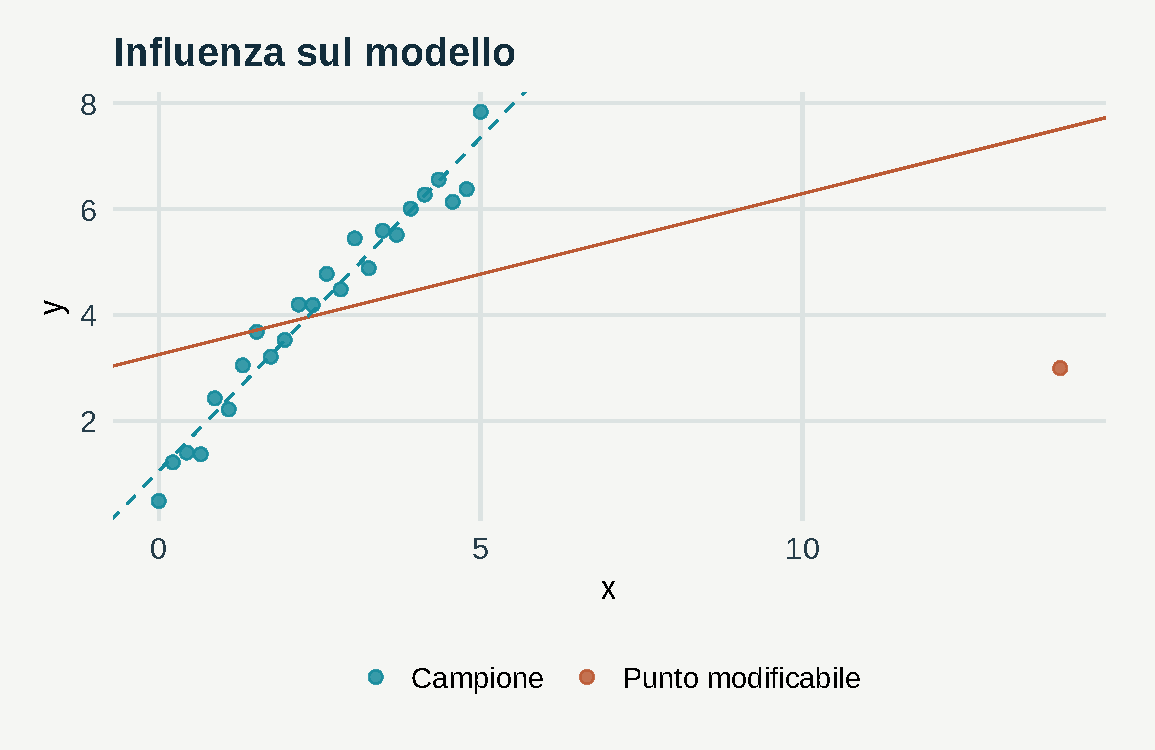
\includegraphics[width=\linewidth,height=5.6cm,keepaspectratio]{Esperimenti/m07-influenza-B.pdf}\par}
\PSmall{Coordinata X del punto: 8 $\to$ 14. Tutti gli altri parametri e il seme sono fissi.}
}};
\node[anchor=north west,inner sep=0] at([xshift=10.85cm,yshift=-2.12cm]current page.north west){\Colonna{8.16cm}{\PLabel{Confronto fra gli scenari}
{\fontsize{10.2}{12.8}\selectfont\begin{tabular}{@{}>{\raggedright\arraybackslash}p{0.48\linewidth}@{\hspace{.13cm}}>{\raggedright\arraybackslash}p{0.224\linewidth}@{\hspace{.13cm}}>{\raggedright\arraybackslash}p{0.224\linewidth}@{}}\toprule Grandezza & A & B\\[2.3pt]
\midrule 
Leva del punto & 0,374 & 0,712\\[2.3pt]
Distanza di Cook & 6,36 & 27,2\\[2.3pt]
Pendenza con punto & 0,744 & 0,304\\[2.3pt]
Pendenza senza punto & 1,26 & 1,26\\[2.3pt]
\bottomrule\end{tabular}\par}
\vspace{.25cm}\PBody{Spostando il punto da x = 8 a x = 14 la leva sale da 0,374 a 0,712 e la distanza di Cook da 6,36 a 27,2. La pendenza con il punto scende da 0,744 a 0,304, mentre quella stimata senza il punto resta 1,26.}
}};
\node[anchor=north east,inner sep=0] at([xshift=17.1cm,yshift=-12.04cm]current page.north west){\fontsize{7.7}{9}\selectfont \href{https://marzione00.github.io/Lab_Geo/\#laboratorio/m07-influenza}{\color{Classical}\bfseries Apri il laboratorio · m07-influenza}};
\end{tikzpicture}\end{frame}

\begin{frame}[plain]\hypertarget{slide30}{}
\bookmark[level=1,page=30]{Dal risultato alla relazione}
\begin{tikzpicture}[remember picture,overlay]
\PilotChrome{Dal risultato alla relazione}{SINTESI}{30}{Riporta stima, unità, scala logaritmica e i due intervalli con le condizioni di ciascuno.}
\node[anchor=north west,inner sep=0] at([xshift=.96cm,yshift=-2.12cm]current page.north west){\Colonna{9.40cm}{\PLabel{Domanda di partenza}
\PBody{Come varia la permeabilità di una carota con la frazione areale dei suoi pori?}
\PLabel{Risultato da discutere}
\PBody{La pendenza stimata è circa −0,0855 per punto percentuale di area, pari a un fattore 0,821 fra medie geometriche della permeabilità. L’intervallo t con dieci gradi di libertà, da −0,226 a 0,055, comprende lo zero; il bootstrap per carote, da −0,202 a −0,009, lo esclude.}
}};
\node[anchor=north west,inner sep=0] at([xshift=10.85cm,yshift=-2.12cm]current page.north west){\Colonna{8.16cm}{\PLabel{Limiti della conclusione}
\PBody{Dodici carote di un dataset storico, prive di località e di età, delimitano il dominio dell’associazione. La frazione areale descrive sezioni bidimensionali, mentre connessione dei pori, tortuosità e gole appartengono alla struttura tridimensionale che la permeabilità riflette.}
\vspace{.4cm}\href{https://marzione00.github.io/Lab_Geo/\#modulo-P02}{\color{Classical}\bfseries Prosegui · P02 · Foraminiferi, coppe e campagne}
}};
\end{tikzpicture}\end{frame}

\begin{frame}[plain]\hypertarget{slide31}{}
\bookmark[level=1,page=31]{Fonti, dati e codice per riprodurre le figure}
\begin{tikzpicture}[remember picture,overlay]
\PilotChrome{Fonti, dati e codice per riprodurre le figure}{RIFERIMENTI}{31}{I risultati numerici si riferiscono ai dati e alle ipotesi dichiarate nel caso.}
\node[anchor=north west,inner sep=0] at([xshift=.96cm,yshift=-2.12cm]current page.north west){\Colonna{9.40cm}{\PLabel{Dati e attribuzioni}
\PBody{Dataset rock del pacchetto datasets di R: quarantotto sezioni di dodici carote di un giacimento petrolifero, con analisi delle immagini di BP Research e Ronit Katz. Gli identificativi di carota sono ricostruiti da blocchi di quattro righe e verificati sui valori distribuiti con R.}
}};
\node[anchor=north west,inner sep=0] at([xshift=10.85cm,yshift=-2.12cm]current page.north west){\Colonna{8.16cm}{\PLabel{Nell’archivio dei sorgenti}
\PBody{Codice contiene i frammenti delle pagine; R contiene lo script P01\_figure.R, che ricostruisce figure e valori dai dati. Esperimenti comprende i programmi dei due scenari, Diagrammi i disegni TikZ modificabili, Scena il modello Blender della copertina.}
\vspace{.4cm}\href{https://marzione00.github.io/Lab_Geo/\#modulo-P01}{\color{Classical}\bfseries Apri la spedizione P01 su GeoStat Lab}
}};
\end{tikzpicture}\end{frame}
\end{document}
